\documentclass[english,12pt,a4paper]{book}

\usepackage[utf8]{inputenc}
\usepackage[english]{babel}
\usepackage[T1]{fontenc}
\usepackage{ragged2e,anyfontsize}
\usepackage{etex}
\usepackage{amsmath,bm,amssymb,amsthm,amsfonts}
\usepackage{mathtools}
\usepackage[titletoc]{appendix}
\usepackage{thmtools}
\usepackage{array}
\usepackage[dvipsnames]{xcolor}
\usepackage[english]{varioref}
\usepackage[numbers]{natbib}
\usepackage[nottoc,numbib]{tocbibind}
\usepackage[font=footnotesize,labelfont={bf},format=hang]{caption}
\usepackage{graphicx}

\usepackage{flafter}
\let\newfloat\relax
\usepackage{float}
\usepackage{caption}

\usepackage{lastpage}
\usepackage{fancyhdr}
\setlength{\headheight}{15pt}

\usepackage{titlesec, blindtext, color}
\usepackage{etoolbox}
\usepackage{tabularx}
\usepackage[a4paper]{geometry}
\usepackage{a4wide}
\usepackage{parskip}
\usepackage{booktabs}
\usepackage{rotating}
\usepackage{textcomp}
\usepackage{url}
\usepackage{hyperref}
\usepackage{mdframed}

%TikZ
\usepackage{tikz}
\usetikzlibrary{arrows.meta, petri, topaths, automata, calc, patterns, angles, quotes, shapes.geometric}
\usepackage{tkz-berge}
\usepackage[position=top]{subfig}
\usepackage{verbatim}
\usepackage{enumitem} 
\usepackage{centernot}
\usepackage{commath}

\usepackage{pgfplots}
\pgfplotsset{compat=1.12}

\hbadness=10001
\vbadness=10001
\setcounter{secnumdepth}{5}
\bibliographystyle{Bibliografi/vancouver}

\setcitestyle{square}

\addto\captionsdanish{
	\renewcommand\contentsname{Table of Contents}	
	\renewcommand{\bibname}{References}
}


%HEADER
\pagestyle{fancy}
\fancyhf{}
\renewcommand{\chaptermark}[1]{ \markboth{\thechapter.\ #1}{}}
\fancyheadoffset{0pt}

\lhead{\nouppercase\leftmark}
\rhead{Aalborg University}

\renewcommand{\chaptermark}[1]%
        {\markboth{#1}{}}
\renewcommand{\sectionmark}[1]%
        {\markright{\thesection\ #1}}

\lfoot[\fancyplain{}{\bfseries\thepage}]%
    {\fancyplain{}{}}
\rfoot[\fancyplain{}{}]%
    {\fancyplain{}{\bfseries\thepage}}


%KAPITEL
\patchcmd{\chapter}{plain}{fancy}{}{}
\definecolor{gray75}{gray}{0.75}
\newcommand{\hsp}{\hspace{15pt}}
\titleformat{\chapter}[hang]{\huge\bfseries}{\thechapter\hsp\textcolor{gray75}{|}\hsp}{0pt}{\huge\bfseries}
\titlespacing*{\chapter}{0pt}{5pt}{25pt}

\newmdtheoremenv{theo}{Sætning}[section]

% %Sætninger, definitioner, mm.
% \declaretheoremstyle[
%     spaceabove=14pt, 
%     spacebelow=6pt, 
%     headfont=\normalfont\bfseries, 
%     bodyfont = \normalfont,
%     postheadspace=2mm, 
%     headpunct={.}]{mystyle}


% %Sætning    
% \declaretheorem[name={Theorem}, style=mystyle,numberwithin=section]{thmx}
% %Definition
% \declaretheorem[name={Definition}, style=mystyle,sibling=thmx]{defn}
% %Eksempel
% \declaretheorem[name={Example}, style=mystyle,sibling=thmx]{exmp}
% %Lemma
% \declaretheorem[name={Lemma}, style=mystyle,sibling=thmx]{lem}
% %Proposition
% \declaretheorem[name={Proposition}, style=mystyle,sibling=thmx]{pro}
% %Korollar
% \declaretheorem[name={Corollary}, style=mystyle,sibling=thmx]{kor}

\usepackage{framed}
\definecolor{myGray}{HTML}{F9F9F9}

%--------

\renewenvironment{leftbar}[4][\hsize]
{
    \def\FrameCommand{
        {\color{#2}\vrule width #4pt}
        \hspace{-8pt}
        \fboxsep=\FrameSep\colorbox{#3}
    }
    \MakeFramed{\hsize#1\advance\hsize-\width\FrameRestore}
}
{\endMakeFramed}

\usepackage{array}
\usepackage{makecell}

\renewcommand\theadalign{bc}
\renewcommand\theadfont{\bfseries}
\renewcommand\theadgape{\Gape[4pt]}
\renewcommand\cellgape{\Gape[4pt]}


\theoremstyle{definition}
\newtheorem{thm}{Theorem}[chapter]
\newtheorem{lemm}[thm]{Lemma}
\newtheorem{pro}[thm]{Proposition}
\newtheorem{cor}[thm]{Corollary}
\newtheorem{defi}[thm]{Definition}
\newtheorem{conj}[thm]{Conjecture}
\newtheorem{eks}[thm]{Example}

\usepackage{changepage}



%----

\newenvironment{thmx}[1]
    {\begin{leftbar}{black}{myGray}{3}
    \begin{thm}#1\\
        }{
    \end{thm}
    \end{leftbar}
    }
    
\newenvironment{prop}[1]
    {\begin{leftbar}{black}{myGray}{3}
    \begin{pro}#1\\
        }{
    \end{pro}
    \end{leftbar}
    }
    
\newenvironment{lem}[1]
    {\begin{leftbar}{black}{myGray}{3}
    \begin{lemm}#1\\
        }{
    \end{lemm}
    \end{leftbar}
    }
  
\newenvironment{defn}[1]
    {\begin{leftbar}{black}{myGray}{3}
    \begin{defi}#1\\
        }{
    \end{defi}
    \end{leftbar}
    }
    
    \newenvironment{kor}[1]
    {\begin{leftbar}{black}{myGray}{3}
    \begin{cor}#1\\
        }{
    \end{cor}
    \end{leftbar}
    }
    
\newenvironment{exmp}[1]
    {\begin{leftbar}{gray}{white}{2}
    \begin{eks}#1\\
        }{
    \end{eks}
    \end{leftbar}
    }
    \AtEndEnvironment{exmp}{\null\hfill$\Diamond$}%



%Bevis
\newtheoremstyle{beviss}% name of the style to be used
  {0pt}% measure of space to leave above the theorem. E.g.: 3pt
  {14pt}% measure of space to leave below the theorem. E.g.: 3pt
  {}% name of font to use in the body of the theorem
  {0pt}% measure of space to indent
  {\bfseries}% name of head font
  {.}% punctuation between head and body
  { }% space after theorem head; " " = normal interword space
  {\thmname{#1}}
\theoremstyle{beviss}
\newtheorem{bev}{Proof}
\AtEndEnvironment{bev}{\null\hfill$\square$}%

\makeatletter
\pretocmd{\chapter}{\addtocontents{toc}{\protect\addvspace{-2\p@}}}{}{}
\pretocmd{\section}{\addtocontents{toc}{\protect\addvspace{0\p@}}}{}{}
\makeatother

\titlespacing*{\subsection}
{0pt}{1em}{1em}





\newcommand{\EE}{\mathbb{E}}
\newcommand{\RR}{\mathbb{R}}
\newcommand{\OO}{\Omega}
\newcommand{\TT}{\mathcal{T}}
\babelhyphenation[english]{gro-up}
\babelhyphenation[danish]{pro-jekt-rap-port}


\title{}
\author{}
\date{}


\definecolor{dkgreen}{rgb}{0,0.6,0}
\definecolor{gray}{rgb}{0.5,0.5,0.5}
\definecolor{mauve}{rgb}{0.58,0,0.82}

\lstset{frame=tb,
  language=Java,
  aboveskip=3mm,
  belowskip=3mm,
  showstringspaces=false,
  columns=flexible,
  basicstyle={\small\ttfamily},
  numbers=none,
  numberstyle=\tiny\color{gray},
  keywordstyle=\color{blue},
  commentstyle=\color{dkgreen},
  stringstyle=\color{mauve},
  breaklines=true,
  breakatwhitespace=true,
  tabsize=3,
  numbers=left
}

\begin{document}

\pagenumbering{roman}

\newcommand{\clearemptydoublepage}{\newpage{\pagestyle{empty}\cleardoublepage}} 

%  A simple AAU report template.
%  2013-03-06 v. 1.0.0
%  Copyright 2010-2013 by Jesper Kjær Nielsen <jkn@es.aau.dk>
%
%  This is free software: you can redistribute it and/or modify
%  it under the terms of the GNU General Public License as published by
%  the Free Software Foundation, either version 3 of the License, or
%  (at your option) any later version.
%
%  This is distributed in the hope that it will be useful,
%  but WITHOUT ANY WARRANTY; without even the implied warranty of
%  MERCHANTABILITY or FITNESS FOR A PARTICULAR PURPOSE.  See the
%  GNU General Public License for more details.
%
%  You can find the GNU General Public License at <http://www.gnu.org/licenses/>.
%
\pdfbookmark[0]{Front page}{label:frontpage}%
\begin{titlepage}
  \addtolength{\hoffset}{0.5\evensidemargin-0.5\oddsidemargin} %set equal margins on the frontpage - remove this line if you want default margins
  \noindent%
  %\vspace{4cm}
  \begin{tabular}{@{}p{\textwidth}@{}}
    %\vspace{5cm}
    \toprule[2pt]
    \midrule
    \vspace{0.4cm}
    \begin{center}
    \Huge{\textsc{Finite Element Model}}
    \end{center}
    \vspace{0.4cm}
  %  \\
   \begin{center}
    %     Undertitel%
    \Large{\textsc{}}% insert your subtitle here
     % }
    \end{center}
    \vspace{0.4cm}\\
    \midrule
    \toprule[2pt]
  \end{tabular}
  \vspace{0.8cm}
  \setlength\fboxsep{0pt}
    %\begin{figure}[ht]
      %  \centering
    %\input{Afsnit/ReptileMotiven.tex}
    %\includegraphics{Billeder/Figurer/ForsideFigur.pdf}
   % \end{figure}
    \setlength\fboxsep{5pt}
  %\begin{center}
    % {Projektrapport 3. semester%Insert document type (e.g., Project Report)
    % }\\
    % \vspace{0.2cm}
    % {Gruppe 4.211%Insert your group name or real names here
    % }
  %\end{center}
  \vfill
\begin{center}
  {\large{Group 5.219b} \\
    {Aalborg University} \\
    {Mathematics} \\}
\end{center}
  
%   \begin{center}
%   Aalborg Universitet\\
%   Institut for Matematiske Fag\\
%   Skjernvej 4A\\
%   DK-9220 Aalborg Øst
%   \end{center}
\end{titlepage}
\clearpage

\thispagestyle{empty}
{\small
\strut\vfill % push the content to the bottom of the page
\noindent Copyright \copyright{} Aalborg University 2020\par
\vspace{0.2cm}
%\noindent Here you can write something about which tools and software you have used for typesetting the document, running simulations and creating figures. If you do not know what to write, either leave this page blank or have a look at the colophon in some of your books.
}
\clearpage

% Dette er LaTeX-versionen af titelbladet for TNB studenterrapporter
% Filen kræver:
% Universitetets logo:  AAU-logo-stud-UK eller AAU-logo-stud-DK
% Synopsis: En fil ved navn synopsis.tex

% Udarbejdet af: Jesper Nørgaard (jesper@noergaard.eu) 10. april 2012

\phantomsection~\pdfbookmark[0]{Titlepage}{titelblad}
\thispagestyle{empty}

\begin{minipage}[t]{0.48\textwidth}
\vspace*{-25pt}			%\vspace*{-9pt}

\includegraphics[height=4cm]{Formalia/AAU-logo-stud-ENG.png}
\end{minipage}
\hfill
\begin{minipage}[t]{0.48\textwidth}
{\small 
\textbf{Department of Mathematical Sciences}\\
Mathematics\\
Skjernvej 4A \\
9220 Aalborg Øst \\
\href{http://math.aau.dk}{http://math.aau.dk}}
\end{minipage}

\vspace*{1cm}

\begin{minipage}[t]{0.48\textwidth}
\textbf{Title:} \\[5pt]\hspace{2ex}
{Finite Element Method}
\bigskip

\textbf{Project:} \\[5pt]\hspace{2ex}
P6-project
\bigskip

\textbf{Project Period:} \\[5pt]\hspace{2ex}
February 2024-May 2024
\bigskip

\textbf{Project Group:} \\[5pt]\hspace{2ex}
5.216c
\bigskip

\textbf{Participants:} \\ [5pt]\hspace{2ex}%\hspace*{2ex}
Jacob Engberg \\%\hspace*{2ex}
William Dam Høedt-Rasmussen\\%\hspace*{2ex}
Patrick Guldberg \\%\hspace*{2ex}

\textbf{Supervisor:} \\ [5pt]\hspace{2ex}%\hspace*{2ex}
Anton Evgrafov \\
Fynn Jerome Aschmoneit \\

\textbf{Pages:~\pageref{LastPage}} \\ [5pt]\hspace{2ex}
\textbf{Finished:} 23\textsuperscript{nd} of May 2024

\end{minipage}
\hfill
\begin{minipage}[t]{0.48\textwidth}
Abstract: \\[5pt]
\fbox{\parbox{6.8cm}{I denne projektrapport gennemgår vi den basale teori 
for 
`Finite Element Method', som bruges til at approksimere løsninger til partiale differentialligninger med grænsebetingelser på kanten.
For at kunne det har vi beskrevet diverse Hilbert rum, og opsætningen af disse,
samt vurderinger af fejlen af approksimationen.
Afslutningsvis eksaminerer vi et numerisk eksempel ved hjælp af programeringsplatformen FEniCSx.\bigskip}}
\end{minipage}
\hspace*{4ex}

\vfill

{\footnotesize \textit{This paper's content is freely available for everyone, but publication (with references) may only happen with acceptance from the authors.}}
\clearemptydoublepage

\setcounter{page}{1}
\addtocontents{toc}{\vspace{-7mm}}
\section*{Preface}
\addcontentsline{toc}{chapter}{\protect\numberline{}Preface}
% Denne projektrapport er udarbejdet af gruppe 4.212 på 4. semester i forbindelse med P4-projektet på Institut for Matematiske Fag ved det Ingeniør- og Naturvidenskabelige fakultet på Aalborg Universitet.

% Projektets forfattere ønsker at rette en tak til Oliver Wilhelm Gnilke, der har fungeret som vejleder under projektperioden.

This student report has been written by group 5.222 throughout the course of 5\textsuperscript{th} semester during the project period at the Department of Mathematical Sciences at Aalborg University.

The authors would like to express their gratitude to Jesper Møller for supervision during the course of the project period.
\vfill

\subsection*{Signatures}
\begin{tabular}{lcl}
    & &\\
    & &\\
    \rule{7cm}{1pt} & \hspace{0.5cm} & \rule{7cm}{1pt} \\
    \vspace{1.5cm}
    Johan Vester Dinesen & & Kristian Skafte Jensen
\end{tabular}
\vspace{1cm}

\pagebreak
\section*{List of Symbols}
\addcontentsline{toc}{chapter}{\protect\numberline{}List of Symbols}
\begin{center}
\begin{figure}[ht!]
\setlength{\extrarowheight}{10pt}
\begin{tabularx}{\textwidth}{rX}
$(u,v)_0$ &   The scalar/inner product on $L_2(\OO)$, meaning $\int_\OO u(x)v(x) dx =(u,v)_{L_2}$ \\
$\|f\|_0$ & The norm on $L_2(\OO)$, meaning $\sqrt{(f,f)_0}$ \\
$(u,v)_m$ & The scalar/inner product on $H^m(\OO)$, meaning $ \sum_{|\alpha|\leq m}(\partial ^{\alpha}u, \partial ^{\alpha} v)_0 $\\
$\|f\|_m$ & The norm on $H^m(\Omega)$, meaning $\sqrt{\sum_{|\alpha|\leq m}\|\partial ^\alpha f\|_{L_2(\Omega)}^2}$ \\
$|f|_m$ & The semi-norm on $H^m(\Omega)$, meaning $\sqrt{\sum_{|\alpha|= m}\|\partial ^\alpha f\|_{L_2(\Omega)}^2}$ \\
$V'$ & Dual space over $V$\\
$\OO$ & An open subset of $\RR^n$ with piecewise smooth boundary \\
$\partial\OO$ & The boundary of $\OO$\\
$\text{div }f$ & $(\partial f/\partial x_1,\partial f/\partial x_2,\ldots,\partial f/\partial x_n)$ \\
$\mathbf{n}$ & The normal derivative\\
$\mathcal{P}_t$ & $\{ f(x,y) = \sum_{i+k \leq t} c_{ik}x^i y^k \}$, for $i,k\geq 0$; I.e. polynomials of degree $t$ \\
%$\blacktriangleleft$    & Afslutning af definition, sætning, lemma, korollar, proposition og eksempel. \\
%$\blacksquare$          & Afslutning af bevis.
\end{tabularx}
\end{figure}
\end{center}
\vfill
% $a$                     & Skalar $\in\F$ \\
% $f(t)$                  & Forskrift for funktion af én variabel.\\
% $\bm{v}$                & $n\times 1$ vektor. \\
% $\bm{f}(t)$             & Forskrift for vektorfunktion. \\
% $A$                     & $m\times n$ matrix eller matrixfunktion. \\
% $\bm{A}$                & Matrix eller matrixfunktion med søjler stablet "på hinanden", hvormed det bliver en vektor i $\R^{n^2}$.
\pagebreak
\tableofcontents
\addtocontents{toc}{\vspace{0mm}}
\clearemptydoublepage

\pagenumbering{arabic}


\chapter{Introduction}
When examining complex physical problems, partial differential equations often occur. 
These equations are often difficult and in some case impossible to calculate algebraically.
We therefore approximate the solution numerically.
One way to do this if the Finite Element Method.
This is done by looking at smaller parts of the domain where we can restrict the problem,
from theese restrictions we are able to approximate solutions, 
and by combining theese solutions we can obtain a approximated solution to the original problem, 
this process is called the Finite Element Method.
Furthermore we are able to give an error estimate of the approximated solution, 
which is important when we want to know how accurate our solution is.

%KAPITEL 1
\chapter{Examination of Partial Differential Equations}

The theory of Finite Element Theory (FEM) springs from a 
wish to solve Partial Differential Equations (PDE's) 
which may or may not have be analytically solvable. 
To do this, we introduce the kind of PDE's we will 
be working with, introducing the forms of the 
problems, and examining the spaces of solutions. 
In this chapter, we will always be working with 
equations with $n$ variables, and $\Omega$ will be 
an open subset of $\RR^n$ with a piecewise smooth boundary.
The PDE which we start with is a second order PDE, 
with the following form.
\begin{equation}
	f(x) = c(x) u + \sum_{i=1}^{n}b_i(x)u_{x_{i}}
	- \sum_{i,k=1}^{n}a_{ik}(x)u_{x_i x_k}\label{eq:pde_order2_n}
\end{equation}
The coefficients in (\ref*{eq:pde_order2_n}) can be 
organized nicely in a vector containing every $b_i$ 
in $b(x)$
and a matrix $A(x)$ containing every $a_{ik}$.
Assuming $u$ in (\ref*{eq:pde_order2_n}) is sufficiently 
smooth, then $u_{x_i x_k} =u_{x_k x_i} $, and $A(x)$ is 
symmetric. 
We use $A(x)$ to define the type of equation we are working 
with, and therefore to characterize the problem we are 
working with.
\begin{defn}{Classification of a PDE}
	The Equation (\ref{eq:pde_order2_n}) is classified as follows:
	\begin{itemize}
		\item Elliptic at $x$, if $A(x)$ is positive definite
		\item Hyperbolic at $x$, if $A(x)$ has one negative and $n-1$ eigenvalues
		\item Parabolic at $x$, if $A(x)$ is positive semidefinite, not positive definite, and rank$([A(x), b(x)])=0$
	\end{itemize}

	If, for every element in the domain of a function, the function is elliptic, hyperbolic, or parabolic, the function itself is called it.
\end{defn}

%
\begin{defn}{\quad}
	The general linear partial differential equation of second order in $n$ variables $x=(x_1,\ldots,x_n)$ has the form
	\begin{equation}
		-\sum_{ i, k = 1 }^n a_{ ik } (x) u_{ x_i x_k } + \sum_{ i = 1 }^n b_i (x) u_{ x_i } + c (x) u = f (x).
		\label{eq:generalPDE}
	\end{equation}
\end{defn}

\begin{defn}{Classification of a PDE}
	The equation~\eqref{eq:generalPDE} is classified as
		\begin{itemize}
			\item elliptic at $x$, if $A(x)$ is positive definite,
			\item hyperbolic at $x$, if $A(x)$ has one negative and $n-1$ eigenvalues and
			\item parabolic at $x$, if $A(x)$ is positive semidefinite, not positive definite, and rank$([A(x), b(x)])=0$.  
		\end{itemize}
	
	If, an equation holds the above conditions for all points of the domain, the equation is called elliptic, hyperbolic or parabolic respectively. 
	\end{defn}
The theory of FEM stems from elliptic PDE's, so we will start by
describing these problems for elliptic PDE's.
\begin{defn}{Partial Differential Operator}~\label{def:pde_operator}
    Let $L$ denote the Partial Differential Operator defined as
    \begin{equation}
        Lu = - \sum_{i,k=1}^n \partial_i(a_{ik} \partial_k u)+ a_0u.
    \end{equation}
    Where $a_{ik}$ are entries in a matrix denoted $A(x)$.
\end{defn}
The ellipticity requirement in Definition~\ref{def:pde_classification} only 
makes demands on the coefficients for the second order partial derivatives, 
and we will ignore the other parts for now. Unless otherwise stated, $L$ is 
always defined as in Definition~\ref{def:pde_operator}.

\section{Hilbert Spaces}
When working with variational problems and the finite 
element method, the end goal is to arrive at some function.
The setup in which we work is therefore spaces of function. 
It is often the case that a classical solution to a given PDE can 
not be found. 
So we define a "weak derivative" using Lebesgue integrals, meaning 
the derivative exists in some strict mathematical sense. 

To use these integrals, we define $L_2(\Omega)$, which are all 
function $f$ over $\Omega$ such that 
\begin{equation*}
   \int_\Omega f^2 dx < \infty. 
\end{equation*}
We use this space to define a weak derivative.
\begin{defn}{Weak derivative}
    A function $f \in L_2(\Omega)$ has a weak derivative $g \in L_2(\Omega)$
    if
    \begin{equation*}
        \int_\Omega g(x)\phi(x) dx = (-1)^{|\alpha|}\int_\Omega 
        \partial ^{\alpha}\phi(x) f(x) dx
        \quad\quad \forall \phi \in C^\infty_0(\Omega).
    \end{equation*}
    We then write $g=\partial ^{\alpha}f$.
    \label{def:weak_derivative}
\end{defn}
We will use derivative and weak derivative interchangeably in this 
text.
If the derivative must be the normal, or strong, derivative, we will 
specify. 

We use Definition \ref*{def:weak_derivative} and $L_2(\Omega)$ spaces 
define the Hilbert space we are going to be working with. 
\begin{defn}{Hilbert Space}
   Let $m \geq 0$. Then $H^m(\Omega)$ is 
   \begin{equation*}
    H^m(\Omega) = \{  f \in L_2(\Omega) \mid \partial ^{\alpha}f \in 
    L_2(\Omega) \quad \forall |\alpha| \leq m  \}.
   \end{equation*}
   In other words, $H^m(\Omega)$ is the functions in $L_2(\Omega)$ 
   which contains weak derivatives up degree $m$.
\end{defn}
In \cite{Brezis} one can find a proof for the following theorem, which 
we use for defining a specific subspace.
\begin{thmx}{\quad}
   Let $\OO \subset \RR^n$ be an open set with piecewise smooth boundary, 
   and let $m \geq 0$. Then $C^\infty (\OO) \cap H^m(\OO)$ is dense in 
   $H^m(\OO)$.
   \label{thm:c_dense_in_h}
\end{thmx}
The reason we state Theorem \ref{thm:c_dense_in_h} is that it implies a 
similar relationship for a smaller subset, namely $C^\infty_0(\OO)$, 
continuous differentiable functions with a compact support. So we can 
define it thusly:
\begin{defn}{\quad}
  Let $H_0^m(\OO)$ be the completion of $C^\infty_0(\OO)$ with respect 
  to the Sobolev norm.
\end{defn} 
We can use $H_0^m(\OO)$ to specify when we are working  


SNAK OM $H_0^m$ OG $C_0^{\infty}$. SIDE 29.
\section{Variational Problems and Solutions}
The goal of this section is to start developing the mathematical 
precision to know of the existence of solutions to a PDE, and how to find 
them. 
To do this, we start with a general abstract theorem on how solutions 
behave in certain problems, then we look at a connection between 
classical solutions and solutions of variational problems, a 
theorem regarding uniqueness of solutions, and existence of 
weak solutions.


\begin{thmx}{Characterization Theorem}
\label{thm:charac_theorem}
    Let $V$ be a linear subspace, such that
        \[
            a: VxV \rightarrow \mathbb{R}
        \]
    is a symmetric positive bilinear form, then $a(v,v)>0$ for all $v \in V$, $v \neq 0$. In addition, let
        \[
            \ell: V \rightarrow \mathbb{R}
        \]
    be a linear functional. Then the quantity

        \[
            J(v):=\frac{1}{2} a(v,v) - \langle\ell,v\rangle 
        \]
    optains its minimum over $V$ at $u$ if and only if
        \begin{equation}
        \label{eq:charac}
            a(u,v) = \ell(v) \quad \text{for all } v \in V.
        \end{equation}
    There is at most one solution to~\eqref{eq:charac}.
\end{thmx}

\begin{proof}

    For $u,v \in V$ and $t \in \mathbb{R}$ we have, that
    \begin{align}
        J(u+tv) &= \frac{1}{2} a(u+tv,u+tv) - \langle\ell,u+tv\rangle \nonumber \\
        &= \frac{1}{2} \left( a(u,u) + a(tv,tv) + 2a(u,tv) \right) - \left( \langle \ell,u\rangle + \langle\ell,tv\rangle \right) \nonumber \\
        &= J(u) + t\left( a(u,v) - \langle\ell,v\rangle \right) + \frac{1}{2}t^2a(v,v). \label{eq:charac_proof_J(u+tv)}
    \end{align}

    If $u \in V$ satisfies~\eqref{eq:charac} and $t=1$, then from~\eqref{eq:charac_proof_J(u+tv)} we have, that
    \begin{alignat}{2}
        J(u+v) &= J(u) + \frac{1}{2}a(v,v) \quad &&\text{for all } v\in V  \nonumber \\
        &> J(u) \quad &&\text{for } v \neq 0.
    \end{alignat}
    Thus $u$ is a ubnique minimal point. 

    To prove the opposite way, we assume that $J$ has a minimum at $u$, then for every $v\in V$, the derirative of the function $t \mapsto J(u+tv)$ must vanish at $t=0$. 
    By~\eqref{eq:charac_proof_J(u+tv)} the derirative of $J(u+tv)$ with respect to $t$ can be found using, that
    \begin{align*}
          J(u+(t+h)v) &= J(u) + (t+h) (a(u,v) - \langle \ell,v\rangle) + \frac{1}{2}(t+h)^2 a(v,v) \\
          &= J(u+tv) + h(a(u,v) - \langle \ell,v\rangle) + \frac{1}{2}((h^2+2th)a(v,v)),
    \end{align*}
    thus the derirative is $a(u,v) - \langle \ell,v\rangle$, and~\eqref{eq:charac} then follows.
\end{proof}
Theorem~\ref{thm:charac_theorem} does not guarantee the existence 
of solutions, it only characterizes them. In Theorem~\ref{thm:charac_theorem} we 
also only make assumptions on the linearity of the space. 
It is possible to set up a variational problem such that $J$ does 
not attain its minimum.
To engage with the existence of solutions, we make more assumptions on 
the space in which we work. To do this we work with Hilbert spaces. 
We start by specifying the bilinear form in Theorem~\ref{thm:charac_theorem}.
\begin{defn}{\quad}
   Let $H$ be a Hilbert space. A bilinear form $a : H \times H \to \RR$ is 
   called continuous if there exists some $C > 0$ such that 
   \begin{equation}
    |a(u,v)| \leq C \|u\|\, \|v\| \quad \forall u,v \in H.
   \end{equation} 
   If a bilinear form $a$ is symmetric and continuous, and there exists som $\alpha >0$ such that 
   \begin{equation*}\label{eq:elliptic}
    a(v,v) \geq \alpha \|v\|^2 \quad \forall v \in H,
   \end{equation*}
   $a$ is called elliptic.
 \end{defn}
From this point forward $a$ will be referring to the bilinear form, given by
\begin{equation}
   a(u,v) = \int_\Omega \left[\sum_{i,k} a_{ik}\partial_iu\partial_kv+a_0uv\right]dx,
\end{equation}
unless otherwise stated.

We now use Theorem~\ref{thm:charac_theorem} to show a link between classical 
solutions and solutions of appropriate variational problems.
\begin{thmx}{Minimal Property}
    Every classical solution of the boundary-value problem, given by
\begin{align}
    -\sum_{i,k} \partial_i (a_{ik}\partial_k u) + a_0 u &= f \quad \text{in } \Omega  \\
    u &= 0 \quad \text{on } \partial \Omega,
\end{align}
    is a solution to the variational problem, given by
    \[
        J(v)=\int_\Omega \left [\frac{1}{2}\sum_{i,k} a_{ik} \partial_i v\partial_k v + \frac{1}{2} a_0 v^2 -fv\right ]dx \longrightarrow \min,
    \]
    among all functions in $C^2(\Omega)\cap C^0(\bar{\Omega})$ with zero boundary values. 
\end{thmx}
\begin{proof}
    We start off by applying Green's formula
    \begin{equation}
    \label{eq:Greens_formula}
        \int_\Omega v\partial_i w dx = -\int_\Omega w \partial_i v dx + \int_{\partial \Omega} v w \vec{n}_i ds.
    \end{equation}
    Here we assume $v$ and $w$ to be $C^1(\OO)$ functions, and $\vec{n}_i$ is the $i$'th component of the outward-pointing normal $\vec{n}$.
    Now if we insert $w=a_{ik}\partial_k u$ in~\eqref{eq:Greens_formula}, we get
    \begin{equation}
    \label{eq:Greens_formula_inserted}
        \int_\Omega v\partial_i (a_{ik} \partial_k u) dx = -\int_\Omega a_{ik} \partial_i v v\partial_k u dx,
    \end{equation}
    given that $v=0$ on $\partial \Omega$.
    Now let 
    \begin{equation}
    \label{eq:a(u,v)}
        a(u,v) = \int_\Omega \left[\sum_{i,k} a_{ik} \partial_i u \partial_k v +a_0 uv \right]dx
    \end{equation}
    and
    \begin{equation}
    \label{eq:l(v)}
        \ell(v) = \int_\Omega fv dx.
    \end{equation}
    Then by summing~\eqref{eq:Greens_formula_inserted} over $i$ and $k$ we get that for every $v\in C^1(\Omega) \cap C(\bar{\Omega})$ with $v=0$ on $\partial \Omega$ we have
    \begin{align}
        a(u,v) - \ell(v) &= \int_\Omega v\left[ -\sum_{i,k} \partial_i (a_{ik} \partial_k u) + a_0 u - f \right] dx \label{eq:min_prop_variational_problem}\\
        &= \int_\Omega v [Lu - f] dx \nonumber \\
        &= 0, \nonumber
    \end{align}
    given that $Lu = f$. This property holds if $u$ is a classical solution.
     The minimal property is then implied by Theorem~\ref{thm:charac_theorem}
\end{proof}
The same kind of proof can be used to show that a solution $u$ to 
(\ref{eq:min_prop_variational_problem}) which fulfills 
$u\in C^2(\OO) \cap C^0(\OO)$ is also a classical solution. 
This gives a connection between classical solutions and solutions of 
variational problems. We now proceed to examine the existence of a 
solution.
\begin{thmx}{Lax-Milgram Theorem}
Let $V$ be a closed, convex, non-empty set in a Hilbert space $H$, and let $a:H \times H \rightarrow \mathbb{R}$ be an elliptic bilinear form. Then for every $\ell\in H'$, the variational problem given by
\[
    J(v)=\frac{1}{2} a(v,v) - \ell(v) \longrightarrow \min    
\]
has a unique solution in $V$.\label{thm:lax_milgram}
\end{thmx}

\begin{bev}
    $J$ is bounded from below, since
    \begin{align*}
        J(v) &\geq \frac{1}{2} \alpha \|v\|^2 - \|\ell\| \, \|v\|\\
        &= \frac{1}{2\alpha} {(\alpha \|v\|-\|\ell\|)}^2 - \frac{\|\ell\|^2}{2\alpha} \\
        &\geq - \frac{\|\ell\|^2}{2\alpha}.
    \end{align*}
    We then let $c_1 = \inf\{J(v); v \in V\}$ and ${\{v_n \}}_{n=1}^\infty$ be a minimizing sequence. Then we get 
    \begin{align*}
        \alpha \|v_n-v_m\|^2 &\leq a(v_n-v_m,v_n-v_m) \\
        &= 2a(v_n,v_n) + 2a(v_m,v_m) - a (v_n+v_m,v_n+v_m) \\
        &= 4J(v_n) + 4J(v_m) - 8J(\frac{v_m+v_n}{2}) \\
        &\leq 4J(v_n) + 4J(v_m) - 8c_1. 
    \end{align*}
    By the convexity assumption on $V$, we get that $\frac{1}{2}(v_n + v_m) \in V$, and from that we get the last 
    inequality.
    We now get that ${\{v_n \}}_{n=1}^\infty$ is a Cauchy sequence in $H$ and $u = \lim_{n\rightarrow \infty}v_n$ exists given the fact that $J(v_n),J(v_m)\rightarrow c_1$ implies $\|v_n - v_m\| \rightarrow 0$ for $n,m\rightarrow \infty$.  

    Since $J$ is continuous,
    we see $J(u) = \lim_{n\rightarrow \infty} J(v_n) = \inf_{v\in V} J(v)$.
     Moreover, we also have that $u\in V$, because we assumed $V$ to be closed. 
    Lastly, we need to show that the solution is unique.
     To do that, we assume both $u_1$ and $u_2$ to be solutions of the variational problem. 
    Then we set up a minimizing sequence $u_1,u_2,u_1,u_2,\ldots$, which we know to be a Cauchy sequence from earlier.
     This implies $u_1 = u_2$.
\end{bev}
The Hilbert spaces we are going to be working with are all going to be 
vector spaces, and thus convex by definition. 
We can therefore use Theorem \ref{thm:lax_milgram} without further considerations 
on our spaces.
We can therefore make use of the following corollary to unify our approach.
\begin{kor}{\quad}
   Assume the same as in Theorem \ref{thm:lax_milgram}, except $V=H$. Then 
   the solution $u$ is given by 
   \label{cor:lax_milgram}
   \begin{equation*}
    a(u,v) = \ell(v).
   \end{equation*}
   \vspace{-9mm}
\end{kor}
\begin{bev}
    The proof follows closely the proof for Theorem \ref{thm:lax_milgram}. 
    Simply replace $V$ with $H$, to find the existence and uniqueness of the 
    solution, and use Theorem \ref{thm:charac_theorem} to find the form, as 
    shown in the corollary.
\end{bev}
Theorem \ref{thm:minimal_property}, Theorem \ref{thm:lax_milgram} and Corollary 
\ref{cor:lax_milgram} together shows us, that solving a Dirichlet problem is 
the same as finding the minimum of the corresponding variational problem. 
We can use this in our approach, both theoretically, and computationally.

When working with PDE's the equation shown in Corollary \ref{cor:lax_milgram} 
is called the variational formulation of a boundary condition problem. 
The general gist is to find some trial function $u$ and examine whether this 
is a solution to our problem, by using some test function $v$. 
As in Corollary \ref{cor:lax_milgram}, all the parts involving the trail function 
is grouped into one part, $a$, and the parts only involving the test functions into 
another, $\ell$.
This changes the problem to something easier to approximate and widens the 
space in which we look for solutions.
%https://fab.cba.mit.edu/classes/864.14/text/variational.pdf
%https://www.ljll.fr/ledret/M1English/M1ApproxPDE_Chapter3.pdf
%https://hplgit.github.io/num-methods-for-PDEs/doc/pub/varform/sphinx/._main_varform001.html#abstract-notation-for-variational-formulations

After proving these statements on qualities of a solution, we can now move 
on to discussing the existence of these solutions. We start by looking at 
sufficiently well-defined solutions. 
% TODO Ændre tekst - har vist noget med eksistens og entydighed, kigger på rum af løsningerne
\begin{defn}{\quad}
    The Dirichlet problem with homogeneous boundary conditions,
     (\ref{eq:b_v_problem_homogeneous}), has a weak solution $u\in H_0^1(\OO)$
     if 
     \begin{equation*}
        a(u,v) = (\tilde{f},v)_0 \quad \forall v \in H_0^1(\OO).
     \end{equation*}
     Here $a(u,v)$ is the bilinear from from(\ref{eq:a(u,v)}), 
     and $(\tilde{f},v)_0$ is a linear bounded functional provided $\tilde{f}\in L^2$, and it can therefore be used as $\ell(v)$ in(\ref{eq:l(v)}).
\end{defn}


\begin{thmx}{Existence theorem}
    Let $L$ be a second order uniformly elliptic partial differential operator from~\eqref{eq:Lu}. Then the homogeneous Dirichlet problem,
     (\ref{eq:b_v_problem_homogeneous}), always has a weak solution in $H_0^1(\OO)$. It is a minimum of the variational problem
    \begin{equation}
        \frac{1}{2} a(v,v) - {(f, v)}_0 \rightarrow \text{min}
    \end{equation}
    over $H_0^1(\OO)$.\label{thm:existence_hom_dirichlet}
\end{thmx}

\begin{bev}
    Let $c = \sup\{\left| a_{ik}(x) \right| \; | \; x \in \OO, 1 \leq i,k \leq n\}$. Then by the Cauchy-Schwarz inequality we get
    \begin{align}
    \begin{split}
        \left| \sum_{i,k} \int a_{ik} \partial_i u \partial_k v dx \right| &\leq c \sum_{i,k} \int  \left|  \partial_i u \partial_k v dx\right|\\
        &\leq c \sum_{i,k} {\left[ \int {\left( \partial_i u \right)}^2 dx \int {\left( \partial_k v \right)}^2 dx  \right]}^{1/2} \\
        &\leq C {\left| u \right|}_1 {\left| v \right|}_1 \label{eq:Cuv}
    \end{split}
    \end{align}
    where $C=cn^2$. 
    We also assume $C\geq \sup\{|a_0(x)| \; | \; x\in \Omega\}$ giving us
    \begin{equation}
        \left|\int a_0 u v dx \right| \leq C \int |u v| dx \leq C \|u\|_0 \|v\|_0.  
        \label{eq:estimate_a_0}   
    \end{equation}
    Then by~\eqref{eq:Cuv} and~\eqref{eq:estimate_a_0} we get continuity of $a$.
    Furthermore the uniform ellipticity implies the pointwise estimate %TODO Hvorfor gør den det?
    \[
        \sum_{i,k} a_{ik} \partial_i v \partial_k v \geq \alpha \sum_i {\left( \partial_i v \right)}^2,
    \]
    for $\text{C}^1(\OO)$ functions. Integrating both sides and using $\text{a}_0 \geq 0$ leads to %TODO Er det fordi man fjerner noget i integralet?
    \begin{equation}
        a(v,v) \geq \alpha \sum_i \int_\OO {\left(\partial_i v\right)}^2 dx = \alpha |v|^2_1, \quad \forall v \in H^1(\OO).
        \label{eq:alpha_ellipticity}
    \end{equation}
    %TODO ref Friedrich equivalent
    We know from Friedrichs' Inequality $|\cdot|_1$ and $\| \cdot \|_1$ are equivalent norms on $H_0^1$,
     resulting in $a$ being an $H^1$-elliptic bilinear form on $H_0^1(\OO)$.
    From Theorem~\ref{thm:lax_milgram} there exists a unique weak solution which is also a solution of the variational problem.
\end{bev}


We can use Theorem \ref{thm:existence_hom_dirichlet} to examine the inhomogeneous Dirichlet problem, 
see (\ref{eq:b_v_problem}). From (\ref{eq:b_v_problem_homogeneous}), let 
$\tilde{u} \in C^2(\OO)\cap C^0(\bar{\OO}) \cap H^1(\OO)$ be a function such that 
\begin{equation*}
   \tilde{u} = g \quad \text{on } \partial \OO.
\end{equation*}
To find a weak solution $w \in H_0^1(\OO)$, we use Theorem \ref{thm:existence_hom_dirichlet} and the 
fact that $(L\tilde{u},v) = a(\tilde{u},v)$, to solve (\ref{eq:b_v_problem}), and
we find $u \in H^1(\OO)$ such that 
\begin{align*}
   a(u,v) = (f,v)_0 \quad \forall v &\in H_0^1(\OO) \\
   u-\tilde{u} & \in H_0^1(\OO).
\end{align*}
%TODO Hvorfor u i H^1? Density assumptions?
We now require $a_0(x)$ in the Elliptic PDE to be bounded from below by a positive number. 
Inequality \eqref{eq:alpha_ellipticity} will also be true for smaller $\alpha$, so if 
necessary we can reduce it, and assume 
\begin{equation*}
  a_0(x) \geq \alpha >0 \quad \forall x \in \OO.
\end{equation*}
This gives us the lower bound on $a$ as 
\begin{equation*}
   a(v,v)  \geq \alpha |v|^2_1 + \alpha \|v\|^2_0 = \alpha \|v\|^2_1 \quad \forall v \in H^1(\OO).
\end{equation*}
We can therefore assume from this point on, that $a$ is $H^1$ elliptic.


\section{Neumann Boundary Conditions}
We remind the reader of the bilinear form we are working with,
\begin{equation}
   a(u,v) = \int_\Omega \left(\sum_{i,k} a_{ik}\partial_i u\partial_k v+a_0uv\right)dx.
\end{equation}
We now require $a_0(x)$ in the Elliptic PDE, see~\ref{def:pde_classification}, to be bounded from below by a positive number (and so also in $a$). 
Inequality~\eqref{eq:alpha_ellipticity} will also be true for smaller $\alpha$, so if 
necessary we can reduce it, and assume 
\begin{equation*}
  a_0(x) \geq \alpha >0 \quad \forall x \in \OO.
\end{equation*}
This gives us the lower bound on $a$ as 
\begin{equation*}
   a(v,v)  \geq \alpha |v|^2_1 + \alpha \|v\|^2_0 = \alpha \|v\|^2_1 \quad \forall v \in H^1(\OO).
\end{equation*}
We can therefore assume from this point on that $a$ is $H^1$ elliptic.

\begin{defn}{Neumann Boundary condition}
    Let $\frac{\partial u}{\partial \mathbf{n}}= \mathbf{n}\cdot \nabla u$ be the normal derivative. Then the Neumann boundary condition is given by
    \begin{equation}
        \frac{\partial u}{\partial \mathbf{n}}  = g\quad \text{on } \partial \Omega.
    \end{equation}
\end{defn}
With this definition, we can start looking at the existence of solutions to problems which are defined using this type of condition.
\begin{thmx}{\quad}
   Let $\OO$  be bounded, have a piecewise smooth boundary, and satisfy the~\label{thm:neumann_solution_existence}
   cone condition. Let $f \in L_2( \OO)$ and $g\in L_2(\partial \OO)$.
   There exists a unique $u \in H^1(\OO)$ that solves the variational problem 
   \begin{equation*}
    J(v) = \frac{1}{2}a(v,v) - {(f,v)}_{0,\OO} - {(g,v)}_{0,\partial\OO} \to \min.
   \end{equation*}
   Also, $u \in C^2(\OO)\cap C^1(\bar{\OO})$ if and only if a classical solution 
   of 
   \begin{align}
    Lu &= f \quad \text{ in }\OO, \nonumber \\
    \sum_{i,k}  \mathbf{n}_i a_{ik} \partial_k u &= g \quad \text{ on } \partial \OO, \label{eq:neuman_condition_boundary}
   \end{align}
   exists, in which case these $2$ solutions are the same. Here $\mathbf{n}$ is outward 
   pointing normal on $\partial \OO$, defined almost everywhere.
\end{thmx}
\begin{bev}
   Due to the Trace Theorem,~\ref{thm:trace}, the functional ${(g,v)}_{0,\partial \OO}$ is bounded,
   and thus $ {(f,v)}_{0,\OO} - {(g,v)}_{0,\partial\OO}$ is a bounded linear functional, 
   and since $a$ is $H^1$ elliptic, Theorem~\ref{thm:lax_milgram} gives us the
   uniqueness and existence of $u$.
   Corollary~\ref{cor:lax_milgram} gives us
   \begin{equation}
      a(u,v) = {(f,v)}_{0,\OO} + {(g,v)}_{0,\partial\OO} \quad \forall v \in H^1(\OO). \label{eq:neumann_lax}
   \end{equation}
   We now move on to the ``if and only if'' part of the theorem. Start by 
   assuming $u \in C^2(\OO)\cap C^1(\bar{\OO})$.
   If we look in the interior, and as such at $v \in H^1_0(\OO)$, we get $\gamma (v)=0$ 
   and~\eqref{eq:neumann_lax} simply becomes a a Dirichlet problem where 
   $u$ is used to define the boundary condition, see~\eqref{eq:b_v_problem_homogeneous}.
   On the interior we then have 
   \begin{equation}
    Lu = f \quad \text{ in }\OO, \label{eq:neumann_on_interior}
   \end{equation} 
   which is the first condition in~\eqref{eq:neuman_condition_boundary}.
   We now examine the boundary, and we assume $v\in H^1(\OO)$.
   In the proof of Theorem~\ref{thm:minimal_property}, we used Green's formula,
    \begin{equation} %? Skal dette slettes?
        \int_\Omega v\partial_i w dx = -\int_\Omega w \partial_i v dx + \int_{\partial \Omega} v w \mathbf{n}_i ds.
    \end{equation}
   In that proof we could assume the integral on the boundary to be zero, which 
   we cannot do here. However, with the same arguments regarding summing and substituting, 
   we get
   \begin{equation}
      a(u,v) - {(f,v)}_{0,\OO} - {(g,v)}_{0,\partial\OO} = 
      \int_\OO v[Lu - f] dx + \int_{\partial \OO}
     \left[ \sum_{i,k}  \mathbf{n}_i a_{ik} \partial_k u-g \right]v ds.
     \label{eq:existence_neumann_last_eq}
   \end{equation}
   Using~\eqref{eq:neumann_lax} and~\eqref{eq:neumann_on_interior},
   the last integral in~\eqref{eq:existence_neumann_last_eq} must be $0$.

   Suppose that for some $i$ and $k$ the function $v_0 = \mathbf{n}_i a_{ik} \partial_k u -g$ does 
   not vanish on $\partial \OO$. 
   Then $\int_{\partial\OO}v_0^2ds>0$, and by the density of 
   $C^1(\bar{\OO})$ in $C^0(\bar{\OO})$, there exists a $v\in C^1(\bar{\OO})$
   such that  $\int_{\partial\OO}v_0\cdot vds>0$, which cannot happen, due that 
   what we found using~\eqref{eq:existence_neumann_last_eq}. 
   We therefore have the second condition in~\eqref{eq:neuman_condition_boundary},
   and $u$ is a classical solution of this boundary problem.

   On the other hand, assuming $u$ is a classical solution and satisfy~\eqref{eq:neuman_condition_boundary},
   we see from~\eqref{eq:existence_neumann_last_eq} that $u$ also satisfy~\eqref{eq:neumann_lax}, and is therefore a solution to the variational 
   problem, and by Theorem~\ref{thm:lax_milgram} unique.
\end{bev}
Not all Neumann problems fulfill the assumption that $a_0(x)>0$. For example in the 
Neumann Poisson problem,  
\begin{align}
\label{eq:Neumann_Poisson}
\begin{split}
    -\Delta u &= f \quad \text{in } \Omega, \\
    \frac{\partial u}{\partial \mathbf{n}} &= g \quad \text{on } \partial \Omega.
\end{split}
\end{align}
one can find $a_0(x)=0$. We remedy that by constructing a subspace $V$.
Due to the fact that~\eqref{eq:Neumann_Poisson} only contains derivatives with respect to $u$,
 additive constants independent of $u$ are unimportant.
Thus if $u$ satisfies~\eqref{eq:Neumann_Poisson}, then $u + c$ also satisfies~\eqref{eq:Neumann_Poisson} for any constant $c$.
This means that the solution to~\eqref{eq:Neumann_Poisson} is only unique up to a constant,
 which extends to other equations with Neumann boundary conditions.

It turns out that we can formulate the weak form of this problem by restricting to the subspace $V=\{v\in H^1(\Omega):\int_{\Omega}vdx=0\}$.
Define $a(u,v) = \int_\OO \nabla u \cdot \nabla v dx$. Examining a version of 
the Friedrich inequality, Theorem~\ref{thm:friedrich}, which can be found on 
page 46 of~\cite{Braess}, $a$ can be found to be $V$-elliptic.
We now want to assert that every classical solution to the variational problem in Theorem~\ref{thm:neumann_solution_existence} satisfies~\eqref{eq:Neumann_Poisson}.
To do this, we let $w=\nabla u$. Thus~\eqref{eq:Neumann_Poisson} can be written as
\begin{align}\label{eq:Neumann_Poisson_weak}
\begin{split}
    -\text{div } w &= f \quad \text{in } \Omega, \\
    \mathbf{n}^T w &= g \quad \text{on } \partial \OO.
\end{split}    
\end{align}
From the Gauss Integral Theorem, we have that
\[\int_{\Omega} \text{div } w dx = \int_{\partial \OO} \mathbf{n}^T w ds.\]
Then from~\eqref{eq:Neumann_Poisson_weak} we get
\begin{align}
\begin{split}
%\int_{\Omega} \text{div } w dx &= \int_{\partial \OO} \mathbf{n}^Tw ds \\ 
\int_{\Omega} -f dx &= \int_{\partial \OO} g ds.
\end{split}
\end{align}
The integral used in $V$ is a bounded linear functional, and thus 
$V$ is a closed and linear subspace of a Hilbert space, 
V is complete with respect to the norm, and is therefore also a Hilbert space. 
We can then use Corollary~\ref{cor:lax_milgram} 
 and get $u\in V$, where
\begin{equation}\label{eq:Lax-Milgram_Neumann}
  a(u,v) = {(f,v)}_{0,\Omega} + {(g,v)}_{0,\partial \OO} \quad \forall v\in V.  
\end{equation}
Equation~\eqref{eq:Neumann_Poisson} has now been shown to be true for 
every classical solution of the variational problem for $u\in V$. However, for some 
$f\in H^1(\OO)\setminus V$, we can use the following construction for 
the constant $c$:
\begin{equation*}
    \forall f \in H^1(\OO): \,\, c = \frac{\int_\OO f(x) dx }{\int_\OO 1 dx}.
\end{equation*}
Define $v(x) = f(x) - c$, and then 
\begin{equation*}
    \int_\OO v(x)dx = \int_\OO f(x) dx - c\int_\OO 1 dx = \int_\OO f(x) dx - \frac{\int_\OO f(x) dx }{\int_\OO 1 dx} \int_\OO 1 dx = 0,
\end{equation*}
so $v \in V$. For every $u\in H^1(\OO)\setminus V$ we can find a fitting 
constant such that $u+c \in V$. Every classical solution of the 
variational problem corresponding to a Neumann Boundary condition therefore 
satisfies~\eqref{eq:Neumann_Poisson}, and~\eqref{eq:Neumann_Poisson} becomes the weak formulation.

The end result is we look for the solution $u\in V$, and use test functions 
$v\in H^1(\OO)$.

\begin{thmx}{\quad}
   Let $\OO$  be bounded, have a piecewise smooth boundary, and satisfy the~\label{thm:neumann_solution_existence}
   cone condition. Let $f \in L_2( \OO)$ and $g\in L_2(\partial \OO)$.
   There exists a unique $u \in H^1(\OO)$ that solves the variational problem 
   \begin{equation*}
    J(v) = \frac{1}{2}a(v,v) - {(f,v)}_{0,\OO} - {(g,v)}_{0,\partial\OO} \to \min.
   \end{equation*}
   Also, $u \in C^2(\OO)\cap C^1(\bar{\OO})$ if and only if a classical solution 
   of 
   \begin{align}
    Lu &= f \quad \text{ in }\OO, \nonumber \\
    \sum_{i,k}  \mathbf{n}_i a_{ik} \partial_k u &= g \quad \text{ on } \partial \OO, \label{eq:neuman_condition_boundary}
   \end{align}
   exists, in which case these $2$ solutions are the same. Here $\mathbf{n}$ is outward 
   pointing normal on $\partial \OO$, defined almost everywhere.
\end{thmx}
\begin{bev}
   Due to the Trace Theorem,~\ref{thm:trace}, the functional ${(g,v)}_{0,\partial \OO}$ is bounded,
   and thus $ {(f,v)}_{0,\OO} - {(g,v)}_{0,\partial\OO}$ is a bounded linear functional, 
   and since $a$ is $H^1$ elliptic, Theorem~\ref{thm:lax_milgram} gives us the
   uniqueness and existence of $u$.
   Corollary~\ref{cor:lax_milgram} gives us
   \begin{equation}
      a(u,v) = {(f,v)}_{0,\OO} + {(g,v)}_{0,\partial\OO} \quad \forall v \in H^1(\OO). \label{eq:neumann_lax}
   \end{equation}
   We now move on to the ``if and only if'' part of the theorem. Start by 
   assuming $u \in C^2(\OO)\cap C^1(\bar{\OO})$.
   If we look in the interior, and as such at $v \in H^1_0(\OO)$, we get $\gamma (v)=0$ 
   and~\eqref{eq:neumann_lax} simply becomes a a Dirichlet problem where 
   $u$ is used to define the boundary condition, see~\eqref{eq:b_v_problem_homogeneous}.
   On the interior we then have 
   \begin{equation}
    Lu = f \quad \text{ in }\OO, \label{eq:neumann_on_interior}
   \end{equation} 
   which is the first condition in~\eqref{eq:neuman_condition_boundary}.
   We now examine the boundary, and we assume $v\in H^1(\OO)$.
   In the proof of Theorem~\ref{thm:minimal_property}, we used Green's formula,
    \begin{equation} %? Skal dette slettes?
        \int_\Omega v\partial_i w dx = -\int_\Omega w \partial_i v dx + \int_{\partial \Omega} v w \mathbf{n}_i ds.
    \end{equation}
   In that proof we could assume the integral on the boundary to be zero, which 
   we cannot do here. However, with the same arguments regarding summing and substituting, 
   we get
   \begin{equation}
      a(u,v) - {(f,v)}_{0,\OO} - {(g,v)}_{0,\partial\OO} = 
      \int_\OO v[Lu - f] dx + \int_{\partial \OO}
     \left[ \sum_{i,k}  \mathbf{n}_i a_{ik} \partial_k u-g \right]v ds.
     \label{eq:existence_neumann_last_eq}
   \end{equation}
   Using~\eqref{eq:neumann_lax} and~\eqref{eq:neumann_on_interior},
   the last integral in~\eqref{eq:existence_neumann_last_eq} must be $0$.

   Suppose that for some $i$ and $k$ the function $v_0 = \mathbf{n}_i a_{ik} \partial_k u -g$ does 
   not vanish on $\partial \OO$. 
   Then $\int_{\partial\OO}v_0^2ds>0$, and by the density of 
   $C^1(\bar{\OO})$ in $C^0(\bar{\OO})$, there exists a $v\in C^1(\bar{\OO})$
   such that  $\int_{\partial\OO}v_0\cdot vds>0$, which cannot happen, due that 
   what we found using~\eqref{eq:existence_neumann_last_eq}. 
   We therefore have the second condition in~\eqref{eq:neuman_condition_boundary},
   and $u$ is a classical solution of this boundary problem.

   On the other hand, assuming $u$ is a classical solution and satisfy~\eqref{eq:neuman_condition_boundary},
   we see from~\eqref{eq:existence_neumann_last_eq} that $u$ also satisfy~\eqref{eq:neumann_lax}, and is therefore a solution to the variational 
   problem, and by Theorem~\ref{thm:lax_milgram} unique.
\end{bev}
%! Renskriv til eksemepl
\begin{exmp}{Mixed conditions}
A word on Dirichlet boundary conditions and Neumann boundary 
conditions-these conditions are not mutually exclusive.
It is possible to have a problem where on some parts of the boundary, 
a constant condition is required, and on other parts not.
% ? Dette er måske et dumt eksempel.

Take for example the flow of air in a room with open windows. 
Assume you have a (very powerful) vacuum cleaner,
 and point it up in the air at some fixed point. 
We know the constant flow of air around the mouth of the vacuum cleaner, which 
gives us a Dirichlet condition there, but the flow of air through the 
windows is not constant, and are better described using Neumann conditions.

These kind of problems lead to looking for a solution in a space $V$ such that 
$H^1_0(\OO) \subset V \subset H^1(\OO)$, with any other conditions used such 
that $V$ is an appropriate space.
\end{exmp}


%KAPITEL 2
\chapter{Preliminary Theory}

We now start taking more obvious steps to being able to calculate approximations. 
The idea is essentially to partition the domain $\OO$ into a finite amount 
of subsets, preferably with certain qualities, which we will discuss later. 

Using these subsets, we can define a subspace of $H^m(\OO)$ or $H^m_0(\OO)$ 
with a finite dimension, called $S_h$. The variational problem, $J(v)$, can then be 
solved over this space, since an infinite number of dimensions can make 
computation difficult, or impossible.

There will be $2$ parts; in one part we 
will examine how the solution of $J$ behaves in $S_h$ versus the full space, 
and in the other we will discuss partitioning $\OO$, using a mesh.
The terminology in the literature is as follows: an \emph{element} or \emph{cell} is a 
subset of $\OO$, meaning a geometric object, and a \emph{finite element} is a 
function from $S_h$. When the context makes the meaning clear, we might deviate from 
this convention.
We will start by limiting our discussion to a polygonial $\OO \in \RR^2$, which 
can be partitioned into triangles or quadrilaterals.

The idea of $S_h$ is to solve the same variational problem as in the global case, 
but in a smaller space-meaning solving
\begin{equation*}
    J(v) = \frac{1}{2}a(v,v) - \ell(v) \to \underset{S_h}{\min}.
\end{equation*}
The only difference is in the space we look for a solution, namely $S_h$. From 
earlier theory, we know that the solution is given by 
\begin{equation*}
    a(u_h,v) = \ell(v) \quad \forall v \in S_h.
\end{equation*}
Since we assumed $S_h$ to be finite dimensional, we can let $ \{ \psi_1, \psi_2, \ldots, \psi_N \}$ 
be a basis for $S_h$. Since $\ell$ is a linear functional and $a$ is bilinear, 
$u_h$ can be found using the following weak formulation:
\begin{equation*}
    a(u_h, \psi_i) = \ell(\psi_i) \quad i = 1, 2, \ldots, N.
\end{equation*}
As $u_h \in S_h$, $u_h$ can be found to be a linear combination of the basis-fuctions, with 
coefficients $z_i$, $i=1, 2, \ldots, N$. As $a$ is bilinear, we get the system of 
equations
\begin{equation*}
    \sum_{k=1}^N z_k a(\psi_k,\psi_i) = \ell(\psi_i) \quad i = 1,2,\ldots,N.
\end{equation*}
Letting $a(\psi_i,\psi_j)$ be the $j,i$-entries in a matrix $A$, $z_i$ and $\ell(\psi_i)$ 
be the entries the vectors $z$ and $b$ respectively, this can be written in matrix form 
\begin{equation*}
    Az = b.
\end{equation*}

It can be shown that the matrix $A$ is symmetric and positive definite, when $a$ is an $H^m$-elliptic bilinear form, as follows. 
The symmetry of $A$ follows directly from the symmetry of $a$, as $a$ is $H^m$-elliptic.
To show that $A$ is positive definite, we need to show that $x^T Ax > 0$ for all $x \neq 0$. Thus
\begin{align*}
    x^T Ax &= \sum_{i,j} x_i A_{ik}x_k \\
    &= a\left(\sum_{k} x_k\psi_k,\sum_{i} x_i\psi_i\right) \\
    &= a(u_h,u_h) \geq \alpha \|u_h\|^2 > 0.
\end{align*}
From now on, we will assume for simplicity that $V\subset H^m(\Omega)$ and $a$ is $V$-elliptic. %TODO Uddyb hvad V er

\begin{defn}{Admissible Partition}
   A partition of $\OO$ into triangles or quadrilaterals, using 
   $\mathcal{T} = \{T_1, T_2, \ldots, T_M \}$, is called admissible if:~\label{def:admissible_partition}
   \begin{enumerate}
    \item $ \bar{\OO} = \cup_{i=1}^M T_i$
    \item If $T_i \cap T_j$ is exactly one point, it is a common vertex of 
    $T_i$ and $T_j$
    \item If, for $i\neq j$, $T_i \cap T_j$ is more than one point, it is a 
    common edge of $T_i$ and $T_j$.
   \end{enumerate}
\end{defn}
We further describe these partitions. If every element in $\mathcal{T}$ has points 
which have at most a distance of $2h$, or equivalently a diameter of $2h$, 
we write $\mathcal{T}_h$. %TODO Family of partitions?
\begin{defn}{Finite Element}
    A finite element is a triple $(T, \Pi,\Sigma)$ which has the following properties:
    \label{def:finite_element}
    \begin{enumerate}
        \item $T\subset \RR^d$ is a polyhedron
        \item $\Pi \subset C(T)$ with finite dimension $s$
        \item $\Sigma$ is a set of $s$ linearly independent functionals on $\Pi$. 
        Every $p\in \Pi$ is uniquely defined by the values of the $s$ functionals in $\Sigma$.
    \end{enumerate}
\end{defn}
The vernacular can be extended as follows:
\begin{itemize}
    \item The parts of $\partial T$ which lies in different hyperplanes are called faces
    \item A set of functions in $\Pi$ which form a basis are called shape functions 
    \item $s$ is the number of local degrees of freedom or local dimension
\end{itemize}
\begin{defn}{Affine Family}
    A family of finite element spaces $S_h$ for partitions $\mathcal{T}_h$ of 
    $\OO\subset \RR^d$ is called an affine family if there exists a finite reference
    element $(T_{\text{ref}}, \Pi_{\text{ref}},\Sigma)$, such that, beside the 
    usual properties of a finite element, there exists some affine mappings 
    $F_j:T_{\text{ref}}\to T_j$ such that
    \begin{equation*}
        \forall v \in S_h \,\,\land \,\, \forall x \in T_j:\,\, v(x) = p(F^{-1}_j(x)) \quad 
        p \in \Pi_{\text{ref}}.
    \end{equation*}
    Meaning, when restricting $v\in S_h$ to some $T_j$, we can fully describe 
    $v$ using some affine mapping and an element in $\Pi_{\text{ref}}$.
\end{defn}
\begin{lem}{Cea's Lemma}
    Let the bilinear form $a$ be $V$-elliptic with $H_0^m(\Omega)\subset V \subset H^m(\Omega)$. In addition, let $u$ and $u_h$ be solutions to the variational problem in $V$ and $S_h\subset V$, respectively. Then
    \begin{equation}
        \label{eq:cea}
        \|u-u_h\|_m\leq \frac{C}{\alpha}\inf_{v_h\in S_h} \|u-v_h\|_m.
    \end{equation}
\end{lem}
\begin{bev}
    The way we define $u$ and $u_h$ yields
    \begin{align}
    \begin{split}
        a(u,v)&= \ell(v) \quad \forall v\in V,\\
        a(u_h,v)&=\ell(v) \quad \forall v\in S_h.
    \end{split}
    \end{align}
    We assumed $S_h\subset V$, and we therefore by subtraction get
    \begin{equation}
        a(u,v)-a(u_h,v)=0 \quad \forall v\in S_h.
    \end{equation}
    which by linearity of $a$ yields
    \begin{equation}
        \label{eq:cea_proof}
        a(u-u_h,v)=0 \quad \forall v\in S_h.
    \end{equation}
    Now let $v_h\in S_h$ and $v=v_h-u_h$. Then combining this with \eqref{eq:cea_proof}, we get  
    \begin{equation}
        a(u-u_h,v_h-u_h)=0 \quad \forall v_h\in S_h,
    \end{equation}
    and
    \begin{align*}
        \alpha\|u-u_h\|_m^2&\leq a(u-u_h,u-u_h)\\
        &=a(u-u_h,u-v_h)+a(u-u_h,v_h-u_h)\\ 
        &\leq C\|u-u_h\|_m\|u-v_h\|_m.
    \end{align*}
    Rearranging the inequality yields 
    \begin{equation}
        \|u-u_h\|_m\leq \frac{C}{\alpha} \|u-v_h\|_m,
    \end{equation} 
    and therefore
    \begin{equation}
        \|u-u_h\|_m\leq \frac{C}{\alpha}\inf_{v_h\in s_h} \|u-v_h\|_m.
    \end{equation}
\end{bev}

\begin{thmx}{\quad}
    Let $k\geq1$ and suppose $\Omega$ is bounded. Then a piecewise infinitely differentiable function $v:\bar{\Omega}\rightarrow \mathbb{R}$
    belongs to $H^k(\Omega)$ if and only if $v\in C^{k-1}(\bar{\Omega})$.
\end{thmx}

\begin{proof}
    For simplicity we restrict ourselves to domains in $\mathbb{R}^2$.
   % , and we only prove for $k=1$. The general case follows by induction.\\
%
    Start by assuming $k=1$.
    Assuming $v\in C^0(\bar\Omega)$ we wish to prove $v\in H^1(\OO)$. Let $\mathcal{T}={\{T_j\}}^M_{j=1}$ be a partition of $\Omega$.
    Define the piecewise functions $w_i:\Omega\rightarrow \mathbb{R}$ for $i=1,2$ as $w_i(x)=\partial_i v(x)$ for $x\in\Omega$,
     where the function can take either of the two limiting values on the edges of $T_j$. %FIXIT: Måske uddyb det her lidt mere (Anton svar)
    \\
    Let $\phi\in C^{\infty}_0 (\Omega)$
   %  and using Green's identity on every element $T_j$ we get
   and we get
    \begin{align}
    \begin{split}
    \int_\Omega \phi w_i dxdy &= \sum_j\int_{T_j} \phi \partial_i v dx dy \\
        &= \sum_j \left( -\int_{T_j} \partial_i \phi v dxdy + \int_{\partial T_j} \phi v \mathbf{n}_i ds\right).
    \end{split}
    \end{align}
    The first equality follows from linearity of integrals and qualities of a partition, and the second equality is Greens identity.
    Since $v$ is continious, 
    the integrals over the interior edges cancel out,
    as the normal vectors point in opposite directions.
     The function $\phi$ has compact support, 
     meaning it is zero on the boundary and outside $\OO$. 
     The integrals on the boundary therefore vanish and we are left with
    \begin{equation}
        \int_\Omega \phi w_i dxdy = -\int_\Omega \partial_i \phi v dxdy.
    \end{equation}
    Which by Definition~\ref{def:weak_derivative} implies that $w_i$ is the first order weak derivative of $v$.
    As $v\in C^0(\bar\Omega)$ we get $v \in L_2(\OO)$. These facts together results in $v\in H^1(\OO)$ by definition.

    We now examine the other implication. 
    Assuming $v\in H^1(\OO)$ we wish to show $v \in C^0(\bar{\OO})$. 
    First we examine $v$ in the neighborhood of an edge of an element, and rotate the edge so it lies on the $y$-axis. 
    On the edge we define the interval $[y_1-\delta, y_2+\delta]$ for $y_1$ and $y_2$ on the edge, and $y_1<y_2$, and 
    $\delta > 0$.
    Define the auxiliary function
    \begin{equation}
        \psi (x) = \int_{y_1}^{y_2} v(x,y) dy.
    \end{equation}
    The auxiliary function has the following properties
    \begin{equation}
        \psi ' =\int_{y_1}^{y_2} \partial_1 v dy, \quad \psi(x_2) - \psi(x_1) =\int_{x_1}^{x_2} \psi ' dx.
    \end{equation}
    Suppose $v \in C^{\infty}(\OO)$. From the Cauchy-Scwarz inequality we get
    \begin{align}
        |\psi(x_2) -\psi(x_1)|^2 &= \left| \int_{x_1}^{x_2} \int_{y_1}^{y_2} \partial_1 v dx dy \right|^2\\
        &\leq \left| \int_{x_1}^{x_2} \int_{y_1}^{y_2} 1 dx dy \right| \cdot | v |_{1, \OO}^2\\
        &\leq |x_2 - x_1| \cdot |y_2 - y_1| \cdot | v |_{1, \OO}^2,
    \end{align}
    which is Lipschitz continuity.
    Reusing the same density argument, since $C^\infty(\OO)$ is dense in $H^1(\OO)$, the previous inequality 
    also holds for $v\in H^1(\OO)$.
    The function $\psi$ is thus continious for the entire domain, and at $x=0$. 
    Since $y_1$ and $y_2$ was arbitrarily chosen, it must be true for the entire edge,
    so $v$ is continious on $\OO$. 
    The boundary of $\OO$ will be included in the edges of the elements,
    and therefore we get $v\in C^0(\bar{\OO})$.

    For $k>1$, assume the theorem holds for $k-1$. We can then, by assumption, differentiate 
    $k-1$ times, where the bi-implication holds after each differentiation. 
    After differentiating $k-1$ times, we arrive at the case we have just proven. 
    The theorem is thus true for $k>1$.
\end{proof}

%KAPITEL 3
\chapter{Aproximations and errors}
We have, so far, used the norms $|\cdot|$ and $\|\cdot\|$ defined over $\OO$. 
This becomes too restrictive, as in approximating the solution we examine a 
reference element. The norms will therefore change depending on the constructed 
mesh. We do so using the following definition.
\begin{defn}{\quad}
    Let $\mathcal{T}_h = \{ T_1,T_2,\ldots,T_M\}$ be a partition of $\OO$, and 
    let $m\geq 1$. Then define 
    \begin{equation*}
        \|v\|_{m,h} = \sqrt{\sum_{T_j\in \mathcal{T}_h}\|v\|^2_{m,T_j}}
    \end{equation*}
\end{defn}
We note if $v\in H^m(\OO)$ then $\|v\|_{m,h}=\|v\|_{m,\OO}$.
\begin{defn}{\quad}
    Let a finite element $(T,\Pi, \Sigma)$ be given, with $v\in\Pi$.
    Let $z_i$ be the $s$ points in $T$ that, through all $p\in\Sigma$, 
    uniquely determines the functions in $\Pi$.
    Define $I: H^t \to \mathcal{P}_{t-1}$ as the function which maps $v\in H^t$ 
    to the polynomial which solves 
    \begin{equation*}
        p(z_i) = v(z_i), \quad 1\leq i \leq s.
    \end{equation*}
\end{defn}

\begin{lem}{\quad~\label{lem:6.2}}
Let $\Omega$ be a domain with a Lipschitz continous boundary which satisfies a cone condition. Furthermore, let $t\geq 2$, and suppose $z_1,z_2,\ldots z_s$ are the
$s = t(t+1)/2$ prescribed points in $\bar{\Omega}$ such that the interpolation operator $I:H^t \rightarrow \mathcal{P}_{t-1}$ is well defined.
Then there exists a constant $c$ such that
\begin{equation}
    \|u-Iu\|_t\leq c\|u\|_t\quad \forall u\in H^t(\Omega).
    \label{eq:lem_6.2}
\end{equation}
\end{lem}

\begin{bev}
    We endow $H^t(\Omega)$ with the norm 
    \begin{equation*}
        |||v||| = |v|_t + \sum_{i=1}^s |v(z_i)|.
    \end{equation*}
It can then be shown that the norms $|||\cdot|||$ and $\|\cdot\|_t$ are equivalent on $H^t(\Omega)$. Thus
\begin{align*}
    \|u-Iu\|_t&\leq c|||u-Iu|||\\
    &= c(|u-Iu|_t + \sum_{i=1}^s|(u-Iu)(z_i)|)\\
    &= c|u-Iu|_t \\
    &= c|u|_t.
\end{align*}
This holds due to the fact that $Iu$ is a polynomial of degree $t-1$, which means that $D^{\alpha} Iu = 0 \text{ forall } |\alpha|=0$, thus $(Iu)(z_1)=u(z_i)$.

We now move on to proving one direction of the equivalence of the norms. 
It can be shown that the imbedding $H^t\hookrightarrow H^2 \hookrightarrow C^0$ is continous (see~\cite{Braess} page 49). Thus
\begin{equation*}
    |v(z_i)|\leq c\|v\|_t\quad \text{for } i=1,2,\ldots,s.
\end{equation*} 
and
\begin{equation*}
    |||v|||\leq (1+cs)\|v\|_t.
\end{equation*}
For the opposite direction, suppose 
\begin{equation*}
    \|v\|_t\leq c|||v|||\quad \text{for all } v\in H^t(\Omega)
\end{equation*}
fails for every positive number $c$. Then there exists some sequence $(v_k)$ in $H^t(\Omega)$ such that
\begin{equation*}
    \|v_k\|_t=1,\quad |||v_k|||\leq \frac{1}{k},\quad k=1,2,\ldots
\end{equation*}
Now it can be shown that a subsequence of $(v_k)$ converges in $\in H^{t-1}(\Omega)$ (see~\cite{Braess} page 32). We can therefore assume that $(v_k)$ itself converges, thus $(v_k)$ is a Cauchy sequence in $H^{t-1}(\Omega)$.
This together with the fact that $|v_k|_t\to 0$ and
 %$\|v_k-v_\ell\|_t^2\leq\|v_k-v_\ell\|_{t-1}^2 + (|v_k|_t + |v_l|_t)^2$, 
\begin{align*}
    \|v_k-v_\ell\|_t^2 &= \|v_k-v_\ell\|_{t-1}^2 + |v_k-v_\ell|_t^2 \\
    & \leq\|v_k-v_\ell\|_{t-1}^2 + (|v_k|_t + |v_\ell|_t)^2 ,
\end{align*}
 we get that $(v_k)$ is a Cauchy sequence in $H^t(\Omega)$, and thus converges in $H^t(\Omega)$.
Thus by the continuity, we get 
\begin{equation}
    \|v^*\|_t = 1\quad \text{and }|||v^*|||=0. 
\end{equation}
If $|v^*|_t = 0$ this implies that $v^*$ is a polinomial of degree $t-1$, and from $v^*(z_i)=0$ for $i=1,2,\ldots,s$, we get $v^*=0$. 
This is a contradiction, which proves the equivalence of the norms. %TODO Contradiction af hvad??
\end{bev}

\begin{lem}{Bramble-Hilbert Lemma}
    Let $\Omega$ be a domain with a Lipschitz continous boundary. Suppose $t\geq 2$ and that $L$ is a bounded linear mapping from $H^t(\Omega)$ into a normed linear space $Y$.
    If $\mathcal{P}_{t-1}\subset \ker L$, then there exists a constant $c$ such that
    \label{lem:Bramble-Hilbert}
    \begin{equation}
        \|Lv\|\leq c|v|_t\quad \forall v\in H^t(\Omega).
    \end{equation}
\end{lem}
\begin{bev}
    Let $I:H^t(\Omega)\rightarrow \mathcal{P}_{t-1}$ be an interpolation operator of the same type as in Lemma~\ref{lem:6.2}.
     Then by the same lemma and the fact that $Iv\in\ker L$, we get
    \begin{equation}
        \|Lv\|=\|L(v-Iv)\|\leq \|L\|\cdot\|v-Iv\|_t\leq c\|L\| \cdot |v|_t,
    \end{equation}
    where the constant $c$  is the same as in Equation~\ref{eq:lem_6.2}.~\label{lem:6.3}
\end{bev}
It is sometimes easier to look at a transformed domain, rather than the original, which leads to the introduction of the Transformation Formula.

\begin{thmx}{Transformation Formula\label{thm:transformation}}
    Let $\OO$ and $\tilde{\OO}$ be affine equivalents; meaning 
    there exists some square, nonsingular matrix $B$, such that 
    \begin{align*}
        &F: \tilde{\OO}\to \OO, \\
        &F(\tilde{x}) = x_0 + B\tilde{x},
    \end{align*}
    which is affine and bijective. For $v\in H^m(\OO)$ define 
    $\tilde{v}(\tilde{x}) = v(F(\tilde{x}))$.
    Then there exists some $c$ such that 
    \begin{equation*}
        |\tilde{v}|_{m,\tilde{\OO}} \leq 
        c \frac{\|B\|^m }{\sqrt{|\det(B)|}}|v|_{m,\OO}.
    \end{equation*}
\end{thmx}
Here $\|B\|$ is the operator norm, and in our case can be thought of 
as 
\begin{equation*}
    \|B\| = \sup\{ \| By\| :\|y\| = 1, y \in \RR^n \},
\end{equation*}
as $\tilde{\OO}\subset \RR^n$.
\begin{bev}
   Writing the $m$th derivative as a multilinear form, we get 
   \begin{equation*}
    (D^m\tilde{v}(\tilde{x}))(\tilde{y}_1, \tilde{y}_2, \ldots, \tilde{y}_m )=
    (D^m v(x))(B\tilde{y}_1, B\tilde{y}_2, \ldots, B\tilde{y}_m ).
   \end{equation*} 
We can extract $B$, and get $\|D^m \tilde{v}\|_{\RR^{nm}} \leq \|B\|^m \|D^m v\|_{\RR^{nm}}$.
As 
\[\partial_{i_{1}}\partial_{i_{2}}\ldots \partial_{i_{m}} v = D^m v(e_{i_1},e_{i_2}, \ldots, e_{i_m})\]
is a $nm$ dimensional vector, we get the following;
\begin{align*}
    \sum_{|\alpha| = m} | \partial ^\alpha \tilde{v} |^2 & \leq n^m \max_{|\alpha|=m} |\partial ^\alpha \tilde{v}|^2 \\
    &\leq n^m \|D^m\tilde{v}\|^2 \\
    &\leq n^m \|B\|^{2m}\|D^m v\|^2 \\
    &\leq n^{2m}\|B\|^{2m} \sum_{|\alpha|=m}|\partial ^\alpha v|^2.
\end{align*}
We now wish to integrate; however, under affine linear transformation in integrals, 
we must include the transformation constant, which results in 
\begin{equation*}
    \int_{\tilde{\OO}} \sum_{|\alpha|} | \partial ^\alpha \tilde{v} |^2 d\tilde{x}
    \leq n^{2m}\|B\|^{2m}\int_{\OO} \sum_{|\alpha|=m}|\partial ^\alpha v|^2 |\det B^{-1}| dx.
\end{equation*}
Which, after taking the square root, gives the theorem.
\end{bev}
When using a transformation from one shape-regular grid to another, we do not get extra terms which can be seen by looking at the geometric interpretation.
Let $F:T_1 \to T_2$, defined as $ \hat{x} \mapsto B\hat{x} + x_0$ be a bijective affine mapping. 
We define $\rho_i$ and $r_i$ to be the radius of the largest inscribed circle and the radius of the smallest circle containing $T_i$ respectively.
Given $x \in \mathbb{R}^2$, with $||x|| \leq 2 \rho_1$, find $y_1, z_1$ such that $x = y_1 - z_1$, where $y_1$ and $z_1$ are points in $T_1$. 
Since $F(y_1), F(z_1) \in T_2$, we have that $||Bx|| \leq 2r_2$, thus
\begin{equation}\label{eq:6.9}
    ||B|| \leq \frac{r_2}{\rho_1}.
\end{equation}
\begin{thmx}{\quad\label{thm:6.4}}
    Let $t \geq 2$, and suppose $\mathcal{T}_h$ is a shape-regular triangulation of $\OO$. Then there exists a constant $c$ such that
    \begin{equation}
        \norm{u - I_h u}_{m,h} \leq c h^{t-m} \norm{u}_{t, H^t(\OO)}, \quad \forall u \in H^t(\OO), \quad 0 \leq m \leq t,
        \label{eq:6.5}
    \end{equation}
    where $I_h u$ denotes the interpolation by a piecewise polynomial of degreee $t-1$.
\end{thmx}

\begin{bev}
    For this proof, we use the $r_i$ as the radius of the smallest circle containing $T_i\in \mathcal{T}_h$, 
    and $\rho_i$ as the radius of the largest inscribed circle in $T_i$.
    We start by proving the following inequality;
    \begin{equation}
        ||u-I_h u||_{m,T_j} \leq c h^{t-m} |u|_{t,T_j}, \quad \forall u \in H^t(T_j)
    \end{equation}
    for every triangle $T_j$ of a shape-regular triangulation $\mathcal{T}_h$. 
    By choosing a reference triangle with $\hat{r} = 2^{-1/2}$, $\hat{\rho} = {(2+\sqrt{2})}^{-1}$ and letting $F : \hat{T} \to T$ with $T = T_j \in \mathcal{T}_h$, 
    we can apply Lemma~\ref{lem:6.2} on the reference triangle and using the transformations formula, Theorem~\ref{thm:transformation}, in both directions, we get
    \begin{align}
        \begin{split}
        ||u-I_h u||_{m,T_j} &\leq c ||B^{-1}||^m |\det B |^{1/2} |\hat{u} - I_h \hat{u}|_{m,T_{\text{ref}}} \\
                            &\leq c ||B^{-1}||^m |\det B |^{1/2} c | \hat{u} |_{t,T_{\text{ref}}} \\
                            &\leq c ||B^{-1}||^m |\det B |^{1/2} \cdot c ||B||^t \cdot |\det B |^{1/2} |u|_{t,T}  \\
                         &\leq c {\left( ||B||  \cdot ||B^{-1}|| \right)}^m ||B||^{t-m} |u|_{t,T}.
        \end{split}
    \end{align}
    Furthermore, by shape regularity, $r_i / \rho_i \leq \kappa$ for all $T_i$ in $\mathcal{T}$, and $||B|| \cdot ||B^{-1}|| \leq \left( 2 + \sqrt{2} \right)\kappa$. 
    From Equation~\eqref{eq:6.9} we get $||B|| \leq h/\hat{\rho}\leq 4h$.
    With all this we have
    \begin{equation}
        ||u-I_h u||_{\ell,T_j} \leq c h^{t-\ell} |u|_{t,T}
    \end{equation}
    Lastly by squaring and summing the terms from $\ell$ to $m$ we get the desired result.
\end{bev}

\begin{defn}
    Let $m\geq 1, H^m_0(\Omega\subset V\subset H^m(\Omega))$, and suppose $a(\cdot,\cdot)$ is a $V$-elliptic bilinear form. 
    Then the variational problem
    \begin{equation}
        a(u,v) = {(f,v)}_0\quad \text{for all } v\in V
    \end{equation}
    is called $H^s$-regular provided that there exists a constant $C=(\Omega,a,s)$ such that for every  $f\in H^{s-2m}(\Omega)$,
    there is a solution $u\in H^s(\Omega)$ satisfying
    \begin{equation}
        \|u\|_s\leq c\|f\|_{s-2m}.
    \end{equation}\label{defn:7.1}
\end{defn}

\begin{thmx}{Regularity Theorem}
    Let a be an $H^1_0$-elliptic bilinear form with sufficiently smooth coefficient functions. Then the following holds. 
    \begin{enumerate}
        \item If $\Omega$ is convex, then the Dirichlet problem is $H^2$-regular. 
        \item If $\Omega$ has a $C^s$ boundary with $s\geq 2$, then the Dirichlet problem is $H^s$-regular.
    \end{enumerate}
\end{thmx}

\begin{thmx}{\quad}
    Suppose $\mathcal{T}_h$ is a family of shape-regular triangulations of $\Omega$. Then the finite element approximation $u_h\in S_h = \mathcal{M}^k_0(k\geq 1)$ satisfies
    \begin{align}
        \begin{split}
            \|u-u_h\|_1&\leq ch\|u\|_2\ \\
            &\leq ch\|f\|_0.
        \end{split}
        \label{eq:7.3}
<<<<<<< HEAD
    \end{align}\label{thm:7.3}
\end{thmx}
\begin{bev}
    From the fact $\Omega$ is convex, we get that the problem is $H^2$-regular and that $\|u\|_2 \leq c_1\|f\|_0$.
    From Theorem~\ref{thm:6.4} we get that some $v_h\in S_h$ satisfying 
    \begin{equation}
    \|u-v_h\|_{1,\Omega} = \|u-v_h\|_{1,h} \leq c_2h\|u\|_{2,\Omega}
    \end{equation}
    exists. Now define $c = (1+c_1)c_2c_3/\alpha$, and combining the prior statements with Céa's Lemma~\ref{lem:cea} we obtain Equation~\ref{eq:7.3}.
=======
    \end{align}
\end{thmx}
\begin{bev}
    From the fact $\Omega$ is convex, we get that the problem is $H^2$-regular and that $\|u\|_2 \leq c_1\|f\|_0$.
    From Theorem \ref{thm:6.4} we get that some $v_h\in S_h$ satisfying 
    \begin{equation}
    \|u-v_h\|_{1,\Omega} = \|u-v_h\|_{1,h} \leq c_2h\|u\|_{2,\Omega}
    \end{equation}
    exists. Now define $c = (1+c_1)c_2c_3/\alpha$, and combining the prior statements with Céa's Lemma \ref{lem:cea} we obtain Equation \ref{eq:7.3}.
>>>>>>> origin/Github-guru
\end{bev}
\input{Afsnit/Kapitel3/Aubin–Nitsche.tex}
We use the previous theorem to prove an inequality more relevant to our situation.
\begin{kor}{\quad\label{kor:7.7}}
   Assume $\mathcal{T}_h$ is a family of shape regular triangulations of $\OO$.
   If $u\in H^1(\OO)$ is the solution of the variational problem, then 
   \begin{equation*}
    \|u-u_h\|_0 \leq cCh \|u-u_h\|_1.
   \end{equation*}
   If $f\in L_2(\OO)$ and $u\in H^2(\OO)$, then 
   \begin{equation*}
    \|u-u_h\|_0 \leq cC^2h^2 \|f\|_0.
   \end{equation*}
\end{kor}
\begin{bev}
   We want to use Theorem~\ref{thm:aubin-nitsche}, which we can by 
   the following observations. Set 
    \begin{equation*}
        H = H^0(\OO)=L_2(\OO) \quad \text{and} \quad V = H^1_0(\OO).
    \end{equation*}
    Then $V \subset H$, and the norms 
    \begin{equation*}
        |\cdot| = \|\cdot\|_0 \quad \text{and} \quad \|\cdot\| = \|\cdot\|_1,
    \end{equation*}
    by $\|\cdot\|_0 \leq \|\cdot\|_1$ gives us continuity of the imbedding.
    We then get
    \begin{equation*}
        \|u-u_h\|_0 \leq C \|u-u_h\|_1 \sup_{g\in H} \left \{ \frac{1}{|g|} \inf_{v \in S_h} \|\varphi_g - v\|_1 \right \},
    \end{equation*}
    By shape regularity, we can use Theorem~\ref{thm:7.3} and evaluate 
    \begin{equation*}
        \sup_{g\in H} \left \{ \frac{1}{|g|} \inf_{v \in S_h} \|\varphi_g - v\|_1 \right \}
        \leq ch,
    \end{equation*}
    and Theorem~\ref{thm:aubin-nitsche} implies the result.
\end{bev}
If the variational problem is sufficiently regular,
Corollary~\ref{kor:7.7} gives us a connection between $f$ in our original problem, 
and how big the error of our FEM approximation can be. 
However, the norms used to measure this error does not describe the error at singular points; there still might be points where the error grows uncontrollably large, 
if we just use Corollary~\ref{kor:7.7}. 
To remedy that we introduce the next theorem. 
\begin{thmx}{\quad\label{thm:max_error}}
    Let the $L_\infty$-norm be 
    \begin{equation*}
        \|v\|_{\infty, \OO} = \esssup_{x\in\OO} |v(x)|.
    \end{equation*}
    Then 
    for a $H^2$-regular variational problem with a solution $u$, the following holds;
    \begin{equation}
        \|u-u_h\|_{\infty, \OO}\leq ch|u|_2.
    \end{equation}
\end{thmx}
\begin{bev}
    For a function $v\in H^2(T_{\text{ref}})$, we let $Iv$ be its interpolant in the polynomial space $\Pi_{\text{ref}}$.
    We have that $H^2\subset C^0$ and therefore 
    \begin{equation}
        \|v-Iv\|_{\infty,T_\text{ref}} \leq c|v|_{2,T_\text{ref}}
        \label{eq:7.9}
    \end{equation}
    by Lemma~\ref{lem:Bramble-Hilbert}.
    Now let $u$ be the solution to the variational problem, and $I_h u$ be the interpolant in $S_h$.
    Then we choose an element $T$ in the triangulation, which we without loss of generality assume to be uniform. 
    Let $\hat{u}$ be the affine transformation of $u|_T$ to the reference triangle.
    Then by Equation~\ref{eq:7.9} and the transformation formula,~\ref{thm:transformation};
    \begin{align}
        \begin{split}
            \|u-I_h u\|_{\infty,T} &= \|\hat{u} - I\hat{u}\|_{\infty,T_{\text{ref}}} \\
            &\leq c|\hat{u}|_{2,T_{\text{ref}}} \\
            &\leq ch|u|_{2,T} \\
            &\leq ch|u|_{2,\Omega}.
        \end{split}
    \end{align}
    From taking the maximum over all triangles, we get
    \begin{equation}
        \|u - I_h u \|_{\infty,\Omega} \leq ch|u|_{2,\Omega}.
        \label{eq:7.10}
    \end{equation}
    Then by the transformation formula and Theorem~\ref{thm:inverse}, we can obtain the inverse estimate as
    \begin{equation}
        \|v_h\|_{\infty,\Omega} \leq ch^{-1} \|v_h\|_{0,\Omega} \quad \text{for all } v_h\in S_h.
    \end{equation}
    Then using Theorem~\ref{thm:6.4} and Corollary~\ref{kor:7.7}
    for $u_h-I_h u\in S_h$
    we get
    \begin{align*}
        \|u_h-I_h u\|_{0,\Omega} &= \| (u-I_h u)-(u-u_h)\|_{0,\Omega} \\
        & \leq \| u-I_h u\|_{0,\Omega}+\|u-u_h\|_{0,\Omega} \\
        &\leq ch^2|u|_{2,\Omega}.
    \end{align*}
    We then use the inverse estimate from earlier. Thus 
    \begin{align}
        \|u-u_h\|_{\infty,\Omega} &\leq \|u-I_h u\|_{\infty,\Omega} + \|u_h-I_h u\|_{\infty,\Omega} \\
        &\leq \|u-I_h u\|_{\infty,\Omega} + ch^{-1} \|u_h-I_h u\|_{0,\Omega} \\
        &\leq ch|u|_{2,\Omega} + ch^{-1} ch^2|u|_{2,\Omega}\\ 
        &\leq \tilde{c}h|u|_{2,\Omega},
    \end{align}
    which is the theorem.    
\end{bev}
Theorem~\ref{thm:max_error} gives us, as the observant reader might have guessed, 
a maximum size of the error of our FEM approximation.
If the variational problem is sufficiently regular (meaning $H^2$)
the error should
become smaller as $h$ becomes smaller. 
We have in this chapter focused on the possible error of our FEM approximation, 
and how big it can be. 
When the variational problem is regular, we have found both an upper maximum 
in general for the error, but we have also shown other error estimates, 
if the problem is not that easy to work with.
We now proceed to the next chapter, and examine an implimentation of 
FEM.
We have in this chapter focused on the possible error of our FEM approximation, 
and how big it can be. 
When the variational problem is regular, we have found both an upper maximum 
in general for the error, but we have also shown other error estimates, 
if the problem is not that easy to work with.
We now proceed to the next chapter, and examine an implimentation of 
FEM.

\chapter{Application and numerical examination}

We will in this chapter apply the theory developed throughout the project to a specific example. 
Here we will consider the following problem with Dirichlet boundary conditions.
We wish to study convergence rate 
\begin{equation}
    u = \e^{x+y}\cos(x)\sin(y)+x  \quad\text{on }\Omega \label{eq:app_dirichlet}
\end{equation}



\begin{align}
\begin{split}
    Lu &= f \quad \text{in } \Omega \\
    u &= g \quad \text{on } \partial \Omega,
\end{split}
\end{align}
Note in this example that, for simplicity, we have chosen the solution $u$ to be the same on the boundary as in the domain.
We will use the finite element method to approximate a solution for the problem. In this context we use the framework FEniCS,
which is a computational tool for solving partial differential equations. 

All references in the following section will be refering to the code listed in Appendix~\ref{app:Code}.

There are three big parts. The first is a solver, 
which solves a FEM-problem, using a certain number of cells, and a certain degree of polynomials. 
The second is a function which calculates the error in $L_2$,
which comes directly from~\cite{"fen-tutorial"}. 
The last part is two functions, which loop over 
various numbers of cells and polynomial degrees, 
and outputs a table. 

We start on line 10 by defining our solution $u$ as the function from Equation~\eqref{eq:app_dirichlet},
after which we define two different interpolations of $u$ using the packages "numpy" and "ufl". 
We do this for convience, as numpy are better for numerical apporiximations, and ufl is 
easier to work with in FEniCSx.
Next, we need to define the mesh and the function space we will be working in. 
We do this on line 16-22, where $N$ defines the number of cells in each directions of our mesh, resulting in $N^2$ elements in total.
Then `degree' defines the degree of polynomials we use in each cell.
Next step in the process is to define the space of trial functions 
and the space of test functions, which we do on line 24-26.
In a different situation, these two spaces could have been different.

We then define the boundary condition, which is simply the function $k$, as mentioned earlier.
With the boundary condition established we can move on to defining the bilinear form $a$ and the linear form $L$.
With all this in place, we can now solve the problem using the PETSc interface from FEniCSx. 
After obtaining the solution, we can look at the error, which can be computed using the $L_2$ norm.

%The convergence rate tells us how fast the error decreases as we increase the number of elements in our mesh.
%Ideally we would like the error to decrease as we decrease the mesh size. This corresponds to showing that the error $e=k_e-k_h$ is bounded by $\|e\|\leq Ch^r$, 
%with being the mesh size, $r$ the convergence rate and $C$ some constant independent of $h$.
The convergence rate tells us how fast the error decreases as we increase the number of elements in our mesh and degree of polynomials.
We will show this imperically by computing the error for different mesh sizes and degrees and comparing them. 
In Table~\ref{tab:convergence}, 
the error for five different mesh sizes are shown. 
For each different mesh, the solution have been approximated using polynomials of degree one through ten.
%The table shows the error decreases as we decrease the cell size for all degrees of the polynomials, 
%and smaller sizes of cells increases the convergence rate dramatically. 
%For example, at $h=0.03125$, the error is less than $40$ already at degree $6$, and 
%for $h=0.0625$ to reach the same error, we need a degree of $8$, while bigger cells do not 
%even reach that size of error.
%Besides that, we can observe for a polynomial of degree $10$ the error changes by a factor $10^{-9}$ from a 
%cell size of $0.25$ to $0.015625$. Meanwhile, for a polynomial of degree $5$ the error changes by a 
%factor $10^{-6}$, and for a polynomial of degree $1$ the error changes by a factor $10^{-2}$. 
%The degree of polynomials used to approximate thus affect the error, and convergence rate, greatly, 
%which is in conjunction with both earlier theory and intuition. 
As can be seen in Table~\ref{tab:convergence}, every time the degree of polynomials used in 
approximations are increased by $1$, the error changes with a factor $10^{-1}$ or factor 
$10^{-2}$, while a similar trend can be seen every time the cell size is halved. 

However, when the error is very small, an increase in degree or decrease in cell size results in 
a increase in error; this can for example be seen at $h=0.0625$ from degree $9$ to $10$, and 
at $h=0.0156$ from degree $5$ to $6$. 
Also, for degree $6$, the error also increases as the cell size is halved from $0.0312$ to $0.0156$.
This can be explained both by computational accuracy for 
numbers of this size, meaning rounding error and truncation, and the ratio between the radii of the
inner and outer circles might increase, which can also be a factor here.
\begin{figure}[ht]
    \center~% chktex-file 44
\begin{tabular}{|r|r|r|r|r|r|}
    \hline
    Degree &                    \multicolumn{5}{c|}{Size of $h$}                                   \\
    \hline
    1  &          0.25 &      0.125       &           0.0625 &          0.03125 &         0.015625 \\
    \hline
    2  & 4.67454e+08   &      2.25264e+08 &      7.91207e+07 &      2.20585e+07 &      5.73871e+06 \\
    \hline
    3  & 2.25595e+08   &      7.90539e+07 &      1.13243e+07 &      1.49544e+06 &           190463 \\
    \hline
    4  & 1.26809e+08   &      1.79289e+07 &      1.32999e+06 &           113656 &           7390.8 \\
    \hline
    5  & 5.12053e+07   &      2.95071e+06 &           300970 &          12221.9 &          402.822 \\
    \hline
    6  & 1.60739e+07   &      1.3077e+06  &          49422.9 &          847.042 &          13.3082 \\
    \hline
    7  & 4.90332e+06   &      416519      &          4436.92 &          34.2407 &         0.272078 \\
    \hline
    8  & 2.93235e+06   &      71557.2     &          234.893 &          1.46575 &       0.00644169 \\
    \hline
    9  & 1.41838e+06   &      4687.31     &          38.2869 &         0.105716 &      0.000220462 \\
    \hline
    10 & 432549        &      1346.04     &          4.40185 &        0.0047685 &       1.4813e-05 \\
    \hline
    11 & 70746.3       &      378.437     &         0.270403 &       0.00012822 &      4.77788e-05 \\
    \hline
\end{tabular}
    \caption{Table of convergence rate of errors}\label{tab:convergence}
\end{figure}
There can be some question as to whether using polynomials of degree $10$ and $64^2$ cells over a 
$2$ by $2$ square is computationally practical in other settings. 
This is where an evaluation of physical properties, like observational accuracy, desired precision and other 
factors would come into play.
There also exists algorithms for refining a coarse mesh. It involves finding hanging nodes, triangle 
points which dissects other triangle edges, and splitting the triangles which are dissected. 
However, making cells distorted can cause the error estimates to diverge, as the ratio between the radii of the
inner and outer circles might increase.
\begin{figure}[H]
    \centering
    \begin{subfigure}{.3\textwidth}
        \centering
        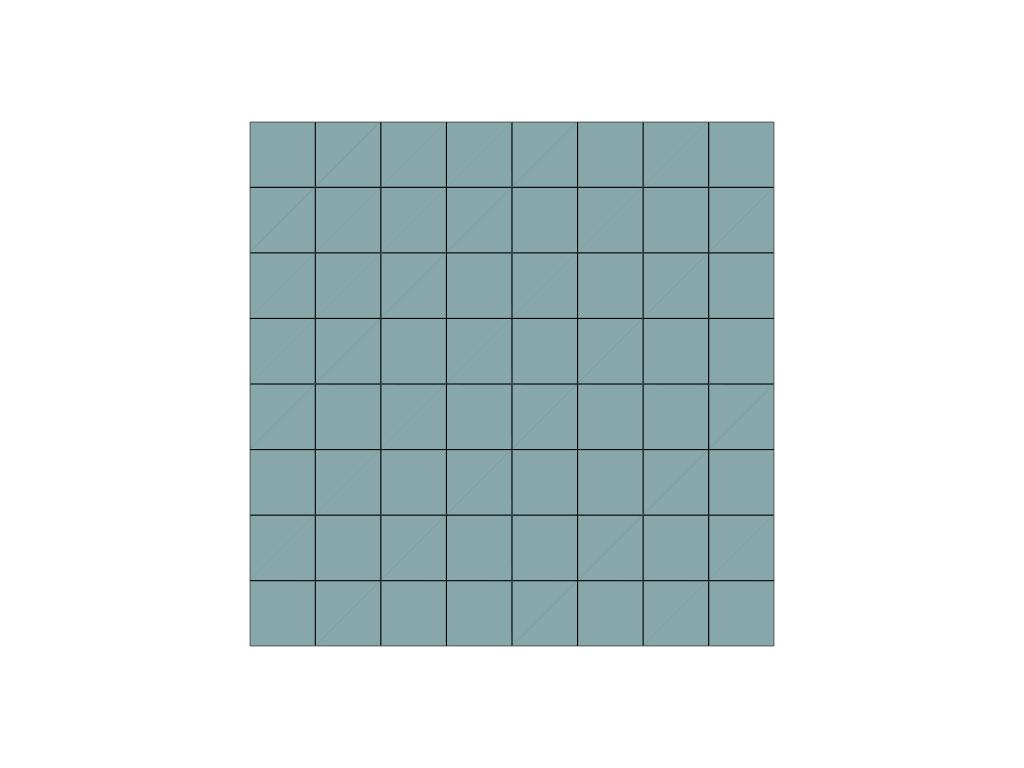
\includegraphics[width=\textwidth]{Afsnit/Application/figurer/screenshot_1.jpeg}
        \caption{Quadrilaterial slicing of domain}~\label{fig:FEM_plot_domain}
      \end{subfigure}
    \begin{subfigure}{.3\textwidth}
        \centering
        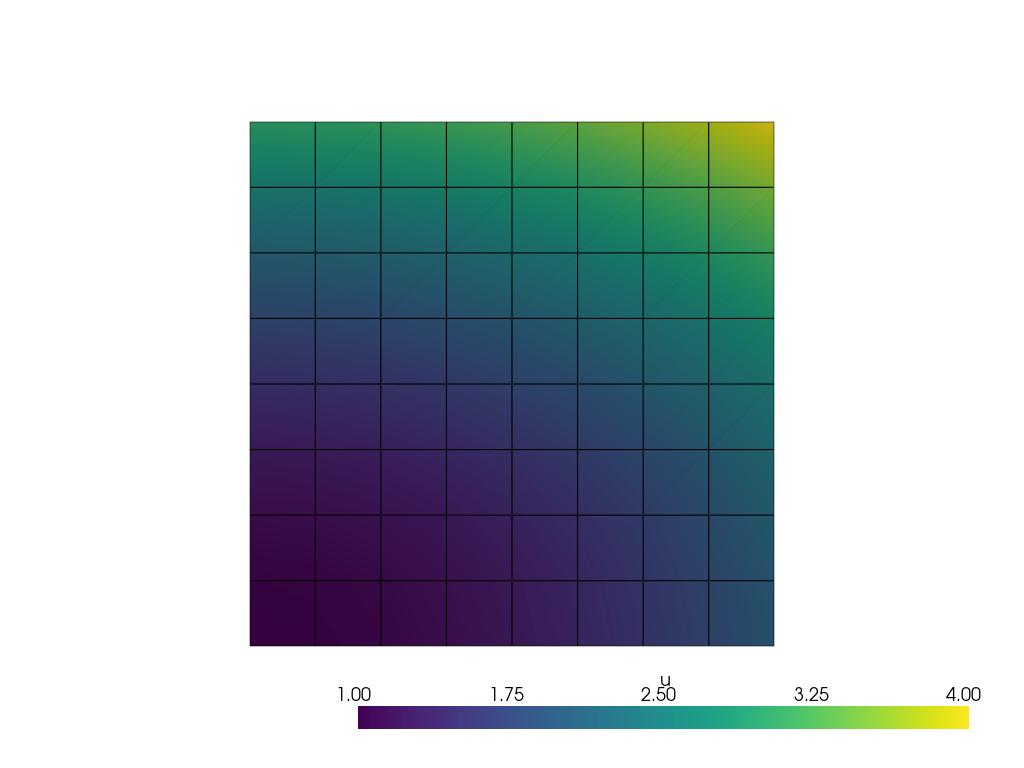
\includegraphics[width=\textwidth]{Afsnit/Application/figurer/screenshot_2.jpeg}
        \caption{Domain colored in accordance to the warping scalar obtained by the solution $u_h$ ranging from 1 to 4}~\label{fig:FEM_plot_warped_domain}
    \end{subfigure}
    \begin{subfigure}{.3\textwidth}
        \centering
        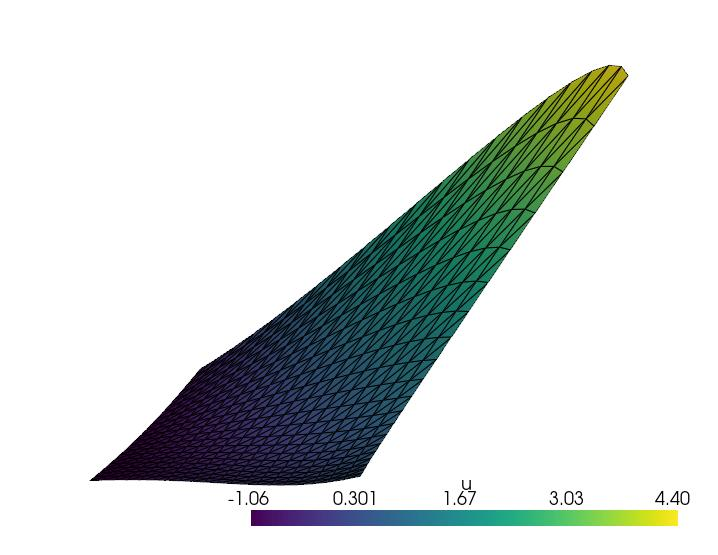
\includegraphics[width=\textwidth]{Afsnit/Application/figurer/screenshot_3.jpeg}
        \caption{The same domain warped with respect to the scalar value, ranging from 1 to 4}~\label{fig:FEM_plot_3D}
    \end{subfigure}
    \caption{Plots of the ?quadrilaterialerised? domain}~\label{fig:FEM_plots}
\end{figure}

As discussed earlier the first step in approximatin the solution to a partial differential equation is do establish a fitting domain. In our example we have chosen a square ranging from $(-1,-1)$ to $(1,1)$.
The domain is then quadrilaterialerised or triangulised depending on the specific scenario, in Plot~\ref{fig:FEM_plot_domain} we have chosen to slice the domain into quadrilaterials, of equal size making the domain regular.
After the domain is sliced and we have estimated the soltion using the nodal points obtained in the quadrilaterials, we can plot the solution over the domain to obtain Plot~\refeq{fig:FEM_plot_warped_domain} where each cell is colored in accordance to the value in the given point.
We can then warp the domain to give a clear look on what exactly our solution looks like in 3D, this is shown in Plot~\refeq{fig:FEM_plot_3D}, where it is also obvious what the visual meaning of a boundary condition, since it is clear the boundary follows the specificied function $1 + x_0^2 + 2x_1^2$.

\chapter{Conclusion}
We have examined how the space containing the solution to a PDE 
with boundary conditions can be constructed, and how a solution can be 
approximated using piecewise polynomials, and by partitioning the domain 
into smaller pieces.
We have focused mostly on partitioning using triangles, though rectangles could 
also have been chosen.
After partitioning the domain we are able to use the Finite Element Method to approximate numerical solutions, 
as we've done in the application section of this project, to 
varying degrees of success, with some behaviour in the convergence rate which were 
not explained.

\bibliography{Bibliografi/Litteratur.bib}

\appendix
\chapter{Code\label{app:Code}}
\section{FEM solver}
\lstinputlisting{FEM.py}
\section{Code to plots}
\lstinputlisting{plot.py}

\end{document}

%TODO: Husk at få Anton til at verificere bevis for 4.11
%TODO: Skal vi fjerne 4.13?
%TODO: Spørg Anton om det giver mening at plotte fejlen fra tabellen for at give et visuelt indtryk af hvor hurtigt fejlen formindskes